%To build the thesis run in this order:
% PDFLateX + BibTex + PDFLateX (x2) + manual edit + PDFLateX (x2)	
% manual edit: Manually modify `main.bbl' by adding \selectlanguage{english} (2nd line) and \selectlanguage{english} (last line) in order to correctly display Latin and Greek characters in the bibliography

\documentclass[11pt,a4paper,english,greek,twoside]{auth-thesis}
\usepackage{epsfig}
%\usepackage[T1]{fontenc}
%\DeclareGraphicsRule{.tif}{bmp}{}{}
\usepackage[explicit]{titlesec}
\usepackage{afterpage}
%\usepackage{algorithmic}
%\usepackage{algorithm}
%\usepackage{amsmath}
\usepackage{mathtools}
\usepackage{amssymb}
\usepackage{amsthm}
\usepackage{array}
\usepackage{color}
\usepackage{courier}
\usepackage{caption}
\usepackage{datetime}
\usepackage{epstopdf}
\usepackage{graphicx}
%\usepackage{IEEEtrantools}
\usepackage{indentfirst}
\usepackage{index}
\usepackage{babel}
\usepackage{listings}
\usepackage{latexsym}
\usepackage{siunitx}
\usepackage{subcaption}
\usepackage{textcomp}
\usepackage{url}
\usepackage{verbatim}
%\usepackage{makeidx}

\newindex{default}{idx}{ind}{Ευρετήριο όρων}
\newindex{en}{edx}{end}{Ευρετήριο αγγλικών όρων}
%\makeindex

% 1.5 spacing
\renewcommand{\baselinestretch}{1.2}

% space between paragraphs
%\setlength{\parskip}{9pt} 

\newcommand\blankpage{%
    \null
    \thispagestyle{empty}%
    \addtocounter{page}{-1}%
    \newpage}
% latin text (and greek text)
%\newcommand{\prg}[1]{\textlatin{\texttt{#1}}}
\newcommand{\tl}[1]{\textlatin{#1}}
\newcommand{\tg}[1]{\textgreek{#1}}

% typeset short english phrases
\newcommand{\en}[1]{\foreignlanguage{english}{#1}}

% typeset inline code
\newcommand{\src}[1]{{\texttt{\en{#1}}}} 

% proper listings caption
\renewcommand{\lstlistingname}{\tg{Κώδικας}}

% typeset a backslash
\newcommand{\bkslash}{\en{\symbol{92}}}

% typeset differential d
\newcommand{\dd}{\mathop{}\,\mathrm{d}}

% create a unit for electrons
\DeclareSIUnit\electrons{\ensuremath{\mathrm{e^-}}}

%typeset infx(a) supx(a) etc
%\newcommand{\infx}[1]{inf_x({#1})}
%\newcommand{\infy}[1]{inf_y({#1})}
%\newcommand{\supx}[1]{sup_x({#1})}
%\newcommand{\supy}[1]{sup_y({#1})}
%\newcommand{\most}{${\cal M}ost$}
%\newcommand{\br}{${\cal B}r$}
\newcommand*\Hide{%
\titleformat{\chapter}[display]
  {}{}{0pt}{\Huge}
\titleformat{\part}
  {}{}{0pt}{}
}
\newtheorem{definition}{Ορισμός}
\newtheorem{proposition}{Πρόταση}
\newtheorem{theorem}{Θεώρημα}
\newtheorem{corollary}{Συμπέρασμα}
\newtheorem{lemma}{Λήμμα}
\newtheorem{example}{Παράδειγμα}
\newtheorem{remark}{Σημείωση}
\newtheorem{notation}{Συμβολισμός}
\newtheorem{law}{Νόμος}
\renewcommand{\thedefinition}{\arabic{chapter}.\arabic{definition}}
\renewcommand{\theproposition}{\arabic{chapter}.\arabic{proposition}}
\renewcommand{\thetheorem}{\arabic{chapter}.\arabic{theorem}}
\renewcommand{\thecorollary}{\arabic{chapter}.\arabic{corollary}}
\renewcommand{\thelemma}{\arabic{chapter}.\arabic{lemma}}
\renewcommand{\theexample}{\arabic{chapter}.\arabic{example}}

%typesetting matlab code
\definecolor{mygreen}{RGB}{28,172,0} % color values Red, Green, Blue
\definecolor{mylilas}{RGB}{170,55,241}
\lstset{language=Matlab,%
	basicstyle=\normalsize\selectlanguage{english}\ttfamily,
    breaklines=true,%
    captionpos=b,                    % sets the caption-position to bottom
    commentstyle=\color{mygreen},%
    emph=[1]{for,end,break},emphstyle=[1]\color{red}, %some words to emphasise
    %emph=[2]{word1,word2}, emphstyle=[2]{style},    
%    escapeinside={\%*}{*)},			% if you want to add LaTeX within your code
    extendedchars=true,
	frame=single,	                   % adds a frame around the code
    identifierstyle=\color{black},	%
%  keepspaces=true,                 % keeps spaces in text, useful for keeping indentation of code (possibly needs columns=flexible)
    keywordstyle=\color{blue},%
    morekeywords=[2]{1}, keywordstyle=[2]{\color{black}},
    morekeywords={matlab2tikz},
  numbers=left,                    % where to put the line-numbers; possible values are (none, left, right)
    numbersep=9pt, % this defines how far the numbers are from the text
    numberstyle={\tiny \color{black}},%  the style that is used for the line-numbers
    showstringspaces=false,%without this there will be a symbol in the places where there is a space
    stringstyle=\color{mylilas},
}

\selectlanguage{greek}
\hyphenation{τμή-μα Επο-μέ-νως}

\title{Ηλεκτρομαγνητική Προσομοίωση ενός \en{Electron Beam Scanner} για Μικρές Δέσμες} 
\author{Ορφέας Αντωνίου}
\supervisor{Νικόλαος Κανταρτζής}
%\TRnumber{} 
%\epitropiF{} 
%\epitropiS{} 


\begin{document}

\selectlanguage{greek}
\maketitle

\frontmatter
\pagenumbering{roman}
\mainmatter
\begin{abstract}
Ο \en{Compact LInear Collider (CLIC)} θα χρησιμοποιεί μια καινοτόμα μέθοδο επιτάχυνσης, στην οποία ενέργεια που εξάγεται από μια υψηλής έντασης δέσμη ηλεκτρονίων σχετικά χαμηλής ενέργειας (τη Δέση Οδηγό), χρησιμοποιείται για την επιτάχυνση μιας χαμηλότερης σε ένταση Κύριας Δέσμης σε πολύ υψηλή ενέργεια.
Η υψηλή ένταση της Δέσμης Οδηγού, με παλμούς που περιέχουν πάνω από $10^{15}$ ηλεκτρόνια, αποτελεί τροχοπέδη στη χρήση συμβατικών μεθόδων μέτρησης προφίλ, όπως τους \en{wire scanners}.
Έτσι, εξετάζονται νέες μη επεμβατικές μέθοδοι μέτρησης προφίλ.

Μια υποψήφια μέθοδος είναι ο Σαρωτής Δεσμών Ηλεκτρονίων (\en{Electron Beam Scanner}). 
Μια δέσμη ανίχνευσης ηλεκτρονίων σε χαμηλή ενέργεια διασχίζει κάθετα την δέσμη του επιταχυντή.
Η δέσμη αυτή αποκλίνει από την πορεία της λόγω των πεδίων της δέσμης του επιταχυντή.
Σαρώνοντας τη δέσμη ανίχνευσης και μετρώντας την απόκλιση της σε σχέση με την αρχική της θέση, το εγκάρσιο προφίλ της δέσμης του επιταχυντή μπορεί να ανακατασκευαστεί.

Αναλυτικές εκφράσεις για την απόκλιση υπάρχουν για την περίπτωση δεσμών μεγάλου μήκους, όπου η κατανομή φορτίου μπορεί να θεωρηθεί σταθερή κατά τη μέτρηση.
Στην παρούσα διπλωματική εργασία εξετάζουμε την επίδοση του σαρωτή δεσμών ηλεκτρονίων σε έναν επιταχυντή όπου το μήκος της δέσμης είναι πολύ μικρότερο από τη διάρκεια σάρωσης της δέσμης ανίχνευσης.
Συγκεκριμένα, η περίπτωση όπου το μήκος της δέσμης είναι μικρότερο από το χρόνο που απαιτεί ένα σωματίδιο της δέσμης ανίχνευσης για να διασχίσει την κύρια δέσμη είναι δύσκολο να μοντελοποιηθεί αναλυτικά.
Αναπτύξαμε ένα περιβάλλον προσομοίωσης που επιτρέπει τη μοντελοποίηση αυτής της περίπτωσης.

   \begin{keywords}
   Σαρωτής Δεσμών Ηλεκτρονίων, προφίλ δέσμης, επιταχυντής \en{CLIC}, μη επεμβατική μέτρηση προφίλ
   \end{keywords}
   
\end{abstract}



\begin{abstracteng}
\tl{The Compact LInear Collider (CLIC) will use a novel acceleration scheme in which energy extracted from a very intense beam of relatively low-energy electrons (the Drive Beam) is used to accelerate a lower intensity Main Beam to very high energy. 
The high intensity of the Drive Beam, with pulses of more than $10^{15}$ electrons, poses a challenge for conventional profile measurements such as wire scanners.
Thus, new non-invasive profile measurements are being investigated.}

\tl{One candidate is the Electron Beam Scanner. A probe beam of low-energy electrons crosses the accelerator beam perpendicularly. 
The probe beam is deflected by the space-charge fields of the accelerator beam. 
By scanning the probe beam and measuring its deflection with respect to its initial position, the transverse profile of the accelerator beam can be reconstructed.}

\tl{Analytical expressions for the deflection exist in the case of long bunches, where the charge distribution can be considered constant during the measurement. 
In this thesis we consider the performance of an electron beam scanner in an accelerator where the bunch length is much smaller than the probe-beam scanning time. 
In particular, the case in which the bunch length is shorter than the time taken for a particle of the probe beam to cross the main beam is difficult to model analytically. 
We have developed a simulation framework allowing this situation to be modelled.}

   \begin{keywordseng}
    \tl{Electron Beam Scanner, beam profile, CLIC accelerator, linear accelerator, non-intercepting profile measurement}
   \end{keywordseng}

\end{abstracteng}
 % abstract and acknowledgements

\tableofcontents
%\listoffigures
%\listoftables
\chapter{Εισαγωγή}


\epigraph{\textit{\en{``It seems probable to me that God, in the beginning, formed matter in solid, massy, hard, impenetrable, moveable particles\ldots "}}}{\en{---Isaac Newton, \textit{Opticks, 1730}}}

\section{Αντικείμενο της διπλωματικής εργασίας}
Ο επιταχυντής \en{CLIC} αποτελεί τον προτεινόμενο γραμμικό επιταχυντή επόμενης γενιάς.
Η καινοτόμα μέθοδος επιτάχυνσης με δύο δέσμες προϋποθέτει μια Δέσμη Οδηγό πολύ υψηλής έντασης.
Λόγω της υψηλής αυτής έντασης, επεμβατικές μέθοδοι μέτρησης της χωρικής έντασης (προφίλ) όπως το \en{wire scanner}\footnote{Το \en{wire scanner} είναι μια ηλεκτρο-μηχανική συσκευή η οποία μετρά το προφίλ μιας δέσμης σε έναν επιταχυντή σωματιδίων χρησιμοποιώντας ένα κινούμενο λεπτό σύρμα.
Καθώς το σύρμα περνά μέσα από τη δέσμη, η αλληλεπίδραση δημιουργεί αλληλουχία δευτερευόντων σωματιδίων, τα οποία με τους κατάλληλους αισθητήρες γίνονται αντιληπτά και επιτρέπουν τη ζητούμενη μέτρηση.} θα καταστρέφονταν.
Έτσι, σχεδιάζονται νέες μη επεμβατικές μέθοδοι για να καλύψουν το κενό αυτό.

Μια τέτοια μέθοδος είναι ο Σαρωτής Δεσμών Ηλεκτρονίων, ή εφεξής \en{``Electron Beam Scanner"}, όπου μία ή περισσότερες δέσμες ανίχνευσης στέλνονται κάθετα προς τη Δέσμη Οδηγό.
Αναλύοντας την απόκλιση αυτών των δεσμών σωματιδίων μας δίνεται η δυνατότητα να υπολογίσουμε το προφίλ της Δέσμης Οδηγού.

Τέτοιες συσκευές έχουν χρησιμοποιηθεί στο παρελθόν σε άλλους επιταχυντές που είχαν συνεχόμενη ροή σωματιδίων, ή πολύ μεγάλες δέσμες.
Η Δέσμη Οδηγός του \en{CLIC} θα έχει δέσμες μήκους μόλις 12 \en{picoseconds}\footnote{Το μήκος της δέσμης σε επιταχυντές μπορεί να εκφραστεί και σε μονάδες χρόνου (π.χ.\ \si{\pico \second}), καθώς οι δέσμες κινούνται πολύ κοντά στην ταχύτητα του φωτός.}, το οποίο αποτελεί επιπλέον πρόκληση για τη χρήση του \en{Electron Beam Scanner}.

Για τη διερεύνηση της επίδρασης των μικρού μήκους δεσμών και για την βελτιστοποίηση του σχεδιασμού του \en{Electron Beam Scanenr}, στην παρούσα διπλωματική εργασία γίνεται μια πλήρης ανάλυση,  ανιχνεύεται η κίνηση δεσμών ανίχνευσης μέσα από το ηλεκτρομαγνητικό πεδίο της Δέσμης Οδηγού και των μερών που την περιβάλλουν. 
Στα πλαίσια αυτής της διερεύνησης χρησιμοποιήθηκε η σουίτα προσομοιώσεων \en{CST}, λόγω των δυνατοτήτων σχετικά με το συνδυασμό ηλεκτρομαγνητισμού και ανίχνευσης σωματιδίων στις προσομοιώσεις.

Επιπλέον, αναζητήθηκαν ποικίλοι τρόποι για την ανίχνευση και τον προσδιορισμό της δέσμης ανίχνευσης και δημιουργήθηκε ο αντίστροφος αλγόριθμος ανακατασκευής του προφίλ της Δέσμης Οδηγού, σε μια προσπάθεια συνδρομής στο σχεδιασμό ενός επιταχυντή επόμενης γενιάς.

\section{Διάρθρωση}
Η παρούσα διπλωματική εργασία είναι οργανωμένη σε πέντε κεφάλαια:

Στο Κεφάλαιο 2 δίνεται το θεωρητικό υπόβαθρο της εργασίας. 
Αυτό περιλαμβάνει μια σύντομη περιγραφή του \en{CERN}, στο οποίο έγινε το μεγαλύτερο κομμάτι της εργασίας, του \en{CLIC}, που αποτελεί τον γραμμικό επιταχυντή που σχεδιάζεται να δημιουργηθεί σε χρονικό ορίζοντα 15 ετών, και παρουσιάζεται και επεξηγείται η λειτουργία του Σαρωτή Δεσμών Ηλεκτρονίων, ή \en{Electron Beam Scanner} όπως θα αναφέρεται.
Σε αυτό το κεφάλαιο αναλύεται και η λειτουργία του \en{Electron Beam Scanner} από μαθηματική σκοπιά, όπως έχει μελετηθεί από την επιστημονική κοινότητα ως τώρα.

Στο Κεφάλαιο 3 παρουσιάζονται οι μέθοδοι προσομοίωσης που χρησιμοποιήθηκαν.
Αρχικά έχουμε μια σύντομη περιγραφή των βασικών εργαλείων που χρησιμοποιήθηκαν, του \en{CST} και του \en{MATLAB}, και στη συνέχεια επεξηγούνται τα στάδια της ανάλυσης που έγινε: ο τρόπος διερεύνησης της επιρροής παραμέτρων του επιταχυντή σε έναν \en{Electron Beam Scanner}, η προσομοίωση της διάταξης εξολοκλήρου στο προσομοιωτικό περιβάλλον του \en{CST} και, τέλος, ο συνδυασμός των δύο εργαλείων, του \en{CST} και του \en{MATLAB}, με σκοπό τη βελτίωση της απόδοσης της προσομοίωσης και της δημιουργίας νέων δυνατοτήτων για προσομοίωση.

Στο Κεφάλαιο 4 παρουσιάζονται και σχολιάζονται τα αποτελέσματα της μελέτης που περιγράφηκε προηγουμένως.

Τέλος, στο Κεφάλαιο 5 δίνονται τα συμπεράσματα, η συνεισφορά αυτής της
διπλωματικής εργασίας, καθώς και προτάσεις για μελλοντική επέκταση της εργασίας.

Στο τέλος της διπλωματικής εργασίας βρίσκονται και 2 παραρτήματα.
Το Παράρτημα Α΄ περιέχει τις μεταφράσεις ξένων όρων που χρησιμοποιήθηκαν στη διπλωματική εργασία, ενώ στο Παράρτημα Β΄ περιγράφεται αναλυτικά το μοντέλο που στήθηκε στο \en{CST}, σε περίπτωση που ο αναγνώστης θελήσει να το αναπαράγει.
\chapter{\selectlanguage{greek}Θεωρητικό υπόβαθρο}
%TODO Write intro

\section{Υπόβαθρο}
\subsection{\selectlanguage{greek}Το \en{CERN}}

To \en{CERN}, διατηρώντας το ακρωνύμιο της αρχικής Γαλλικής ονομασίας του \en{$``$Conseil Européen pour la Recherche Nucléaire$"$}, είναι το μεγαλύτερο σε έκταση πειραματικό κέντρο πυρηνικών ερευνών και ειδικότερα επί της σωματιδιακής φυσικής στον κόσμο. 
Βρίσκεται δυτικά της Γενεύης, στα σύνορα Ελβετίας και Γαλλίας και ιδρύθηκε το 1954 από 12 ευρωπαϊκές χώρες. 
Σήμερα αριθμεί 20 κράτη-μέλη, μεταξύ των οποίων και η Ελλάδα, η οποία είναι και ιδρυτικό μέλος.

\begin{figure}[tph]

\includegraphics[width=0.25\linewidth]{images/CERNlogo}
\centering
\caption{Το λογότυπο του \en{CERN}}
\label{img:CERNlogo}
\end{figure}

Η βασική λειτουργία του \en{CERN} είναι η παροχή επιταχυντών σωματιδίων και άλλων υποδομών απαραίτητων για την έρευνα στον τομέα της φυσικής υψηλών ενεργειών και ως αποτέλεσμα έχουν πραγματοποιηθεί πολυάριθμα πειράματα εκεί, μέσω διεθνών συνεργασιών.

Επίσης, το \en{CERN} αποτελεί τη γενέτειρα του Παγκόσμιου Ιστού (\en{World Wide Web}).
Στην κύρια τοποθεσία του στο \en{Meyrin} βρίσκεται μεγάλη εγκατάσταση ηλεκτρονικών υπολογιστών με ισχυρές υποδομές επεξεργασίας δεδομένων, κυρίως για την ανάλυση των πειραματικών δεδομένων. 
Λόγω της ανάγκης να καταστούν αυτές διαθέσιμες σε εξωτερικούς ερευνητές, υπήρξε ιστορικά ένας σημαντικός κόμβος δικτύου ευρείας περιοχής (\en{Wide Area Network}).

Αρκετά σημαντικά επιτεύγματα στο πεδίο της φυσικής των σωματιδίων έγιναν μέσω πειραμάτων στο \en{CERN}. Αυτά περιλαμβάνουν:
\begin{itemize}
\item 1973: Ανακάλυψη των ουδέτερων ρευμάτων στο θάλαμο φυσαλίδων \en{Gargamelle}.
\item 1983: Ανακάλυψη των μποζονίων $W$ και $Z$ στα πειράματα \en{UA1} και \en{UA2}.
\item 1995: Πρώτη δημιουργία ατόμων αντιυδρογόνου στο πείραμα \en{PS210}.
\item 1999: Ανακάλυψη της άμεσης παραβίασης \en{CP} στο πείραμα \en{NA48}.
\item 2010: Απομόνωση 38 ατόμων αντιυδρογόνου.
\item 2011: Διατήρηση αντιυδρογόνου για πάνω από 15 λεπτά.
\item 2012: Ένα μποζόνιο με μάζα περίπου \SI[per-mode = symbol]{125}{\giga \electronvolt \per  \clight \squared} συνάδει με τον πολυπόθητο μποζόνιο \en{Higgs}.
\end{itemize}


\subsection{\selectlanguage{greek}Ο επιταχυντής \en{CLIC}}


Ο \en{CLIC --- Compact LInear Collider} --- αποτελεί μια μελέτη για ένα μελλοντικό επιταχυντή που θα φτάσει σε πρωτοφανή επίπεδα ενέργειας ηλεκτρόνια και αντισωμάτιά τους, ποζιτρόνια. 
Όταν θα έρχονται σε επαφή μέσω σύγκρουσης, θα αλληλοκαταστρέφονται, απελευθερώνοντας όλη τους την ενέργεια για την παραγωγή νέων σωματιδίων.

\begin{figure}[b]

\includegraphics[trim={12mm 12mm 12mm 12mm},clip=true,width=0.25\linewidth]{images/CLIClogo}
\centering
\caption{Το λογότυπο του \en{CLIC}}
\label{img:CLIClogo}
\end{figure}

Τα ηλεκτρόνια και τα ποζιτρόνια είναι θεμελιώδη σωματίδια και οι συγκρούσεις τους μπορούν να προσφέρουν εξαιρετικά λεπτομερείς πληροφορίες σχετικά με τους νόμους της φύσης. 
Έτσι ο \en{CLIC} θα προσφέρει σημαντικές θεμελιώδεις γνώσεις φυσικής, πέρα από αυτές που είναι διαθέσιμες από το Μεγάλο Επιταχυντή Αδρονίων (\en{Large Hadron Collider --- LHC}) ή από ένα γραμμικό επιταχυντή ηλεκτρονίων/ποζιτρονίων χαμηλότερης ενέργειας, λόγω του μοναδικού συνδυασμού πειραματικής ακρίβειας και υψηλής ενέργειας.

Σε αυτές τις υψηλές ενέργειες, τα ηλεκτρόνια και ποζιτρόνια θα έχαναν ένα τεράστιο μέρος της ενέργειάς τους επιταχυνόμενα σε έναν κυκλικό επιταχυντή σαν τον \en{LHC}. 
Επομένως, τα σωματίδια πρέπει να επιταχυνθούν σε δύο γραμμικούς επιταχυντές που αντικρίζουν ο ένας τον άλλο έτσι, ώστε οι δέσμες να συγκρούονται στον κεντρικό ανιχνευτή. 
Αυτό συνεπάγεται ότι τα σωματίδια πρέπει να αποκτήσουν την ενέργειά τους από ένα και μόνο πέρασμα τους μέσα από τις κοιλότητες επιτάχυνσης.

\begin{figure}[tph]
\includegraphics[width=0.6\linewidth]{images/CLIC-twobeam}
\centering
\caption{Το σύστημα δύο δεσμών του \en{CLIC}}
\label{img:CLICtwobeamscheme}
\end{figure}

Ο \en{CLIC} έχει σχεδιαστεί για να κατασκευαστεί σε στάδια αυξανόμενης ενέργειας για σύγκρουση: ξεκινώντας από \SI{360}{\giga \electronvolt}, περίπου \SI{1.4}{\TeV}, και μέχρι την τελική ενέργεια των \SI{3}{\TeV}. 
Προκειμένου να επιτευχθεί αυτή η ενέργεια με ένα ρεαλιστικό και οικονομικά αποδοτικό τρόπο, η αύξηση της επιτάχυνσης πρέπει να είναι πολύ υψηλή.
Ο \en{CLIC} αποσκοπεί σε επιτάχυνση των \SI[per-mode = symbol]{100}{\mega \volt \per \metre}, 20 φορές υψηλότερη από αυτή του \en{LHC}.

Για να επιτευχθεί αυτό, χρησιμοποιείται μια καινοτόμα μέθοδος επιτάχυνσης, όπου εξάγεται ενέργεια από μια δέσμη πολύ μεγάλης έντασης που περιέχει σχετικά χαμηλής ενέργειας ηλεκτρόνια (Δέσμη Οδηγός) και χρησιμοποιείται για την επιτάχυνση της χαμηλότερης σε ένταση Κύριας Δέσμης (\en{Main Beam}) σε πολύ μεγάλη ενέργεια.

Αυτή η Δέσμη Οδηγός (\en{Drive Beam}) επιβραδύνεται σε ειδικές Διατάξεις Εξαγωγής και Mεταφοράς Ισχύος --- \en{Power Extraction and Transfer Structures (PETS)}, και η παραγόμενη \en{RF} ισχύς μεταφέρεται στην κύρια δέσμη. 
Αυτό οδηγεί σε μια πολύ απλή διάταξη σήραγγας χωρίς ενεργά \en{RF} μέρη (δηλ. \en{klystrons}).

\begin{figure}[tph]
\includegraphics[width=\linewidth]{images/CLIC-layout}
\centering
\caption{Το σχεδιάγραμμα του \en{CLIC}}
\label{img:CLIClayout}
\end{figure}

\begin{figure}[tph]
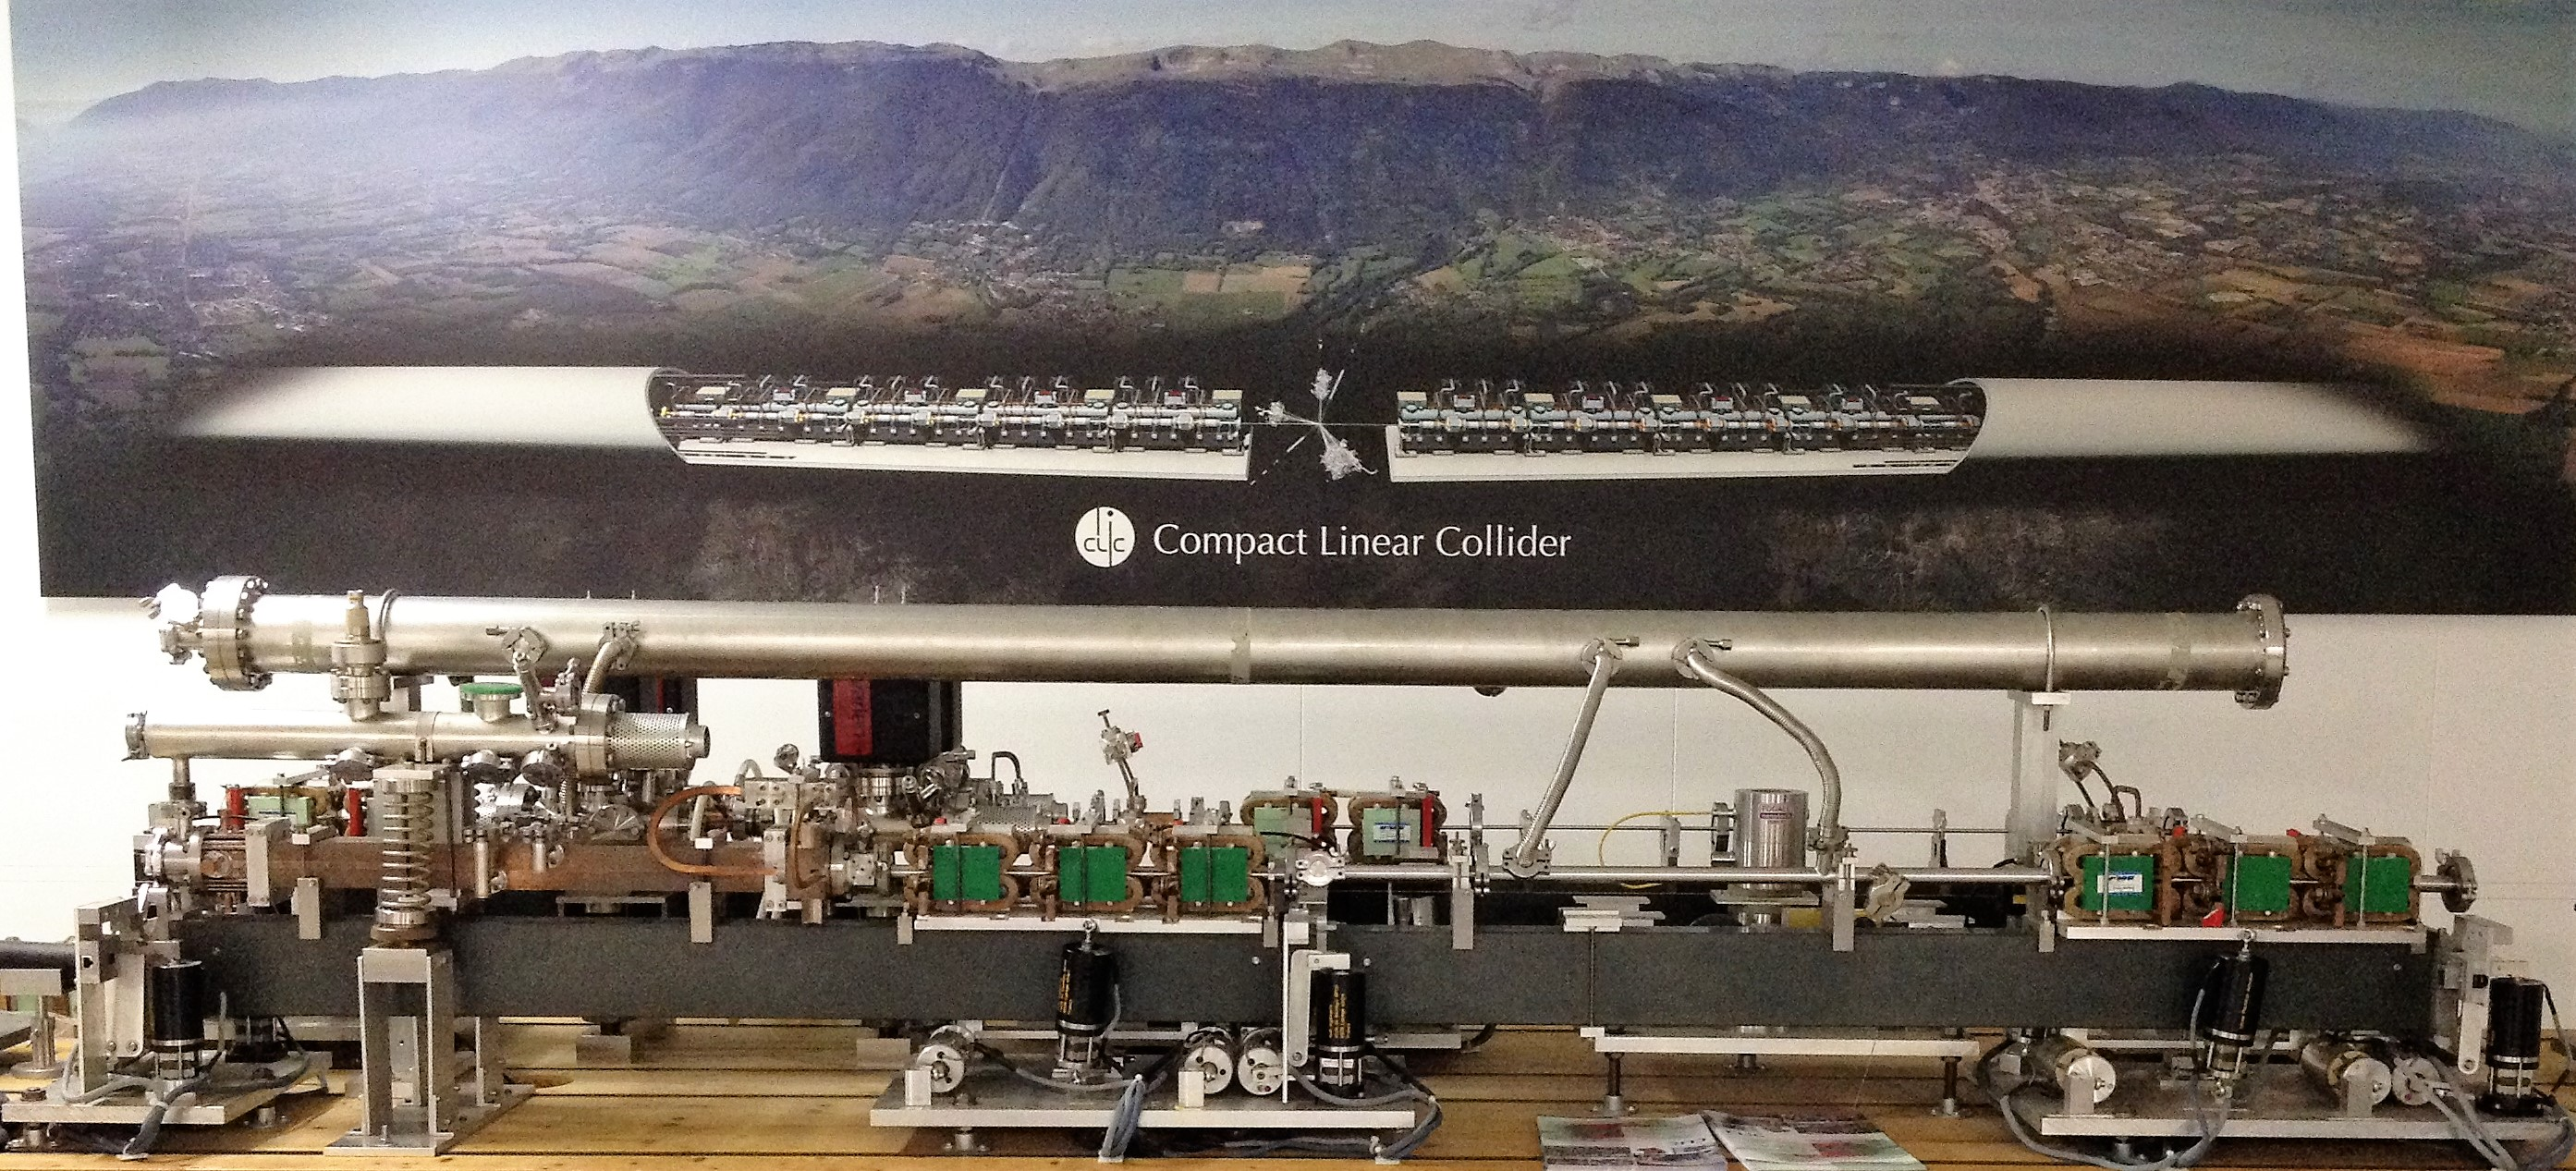
\includegraphics[width=\linewidth]{images/CLIC-maquette}
\centering
\caption[Η μακέτα του \en{CLIC}]{Η μακέτα του \en{CLIC} που βρίσκεται στο κτήριο δοκιμών \en{CLIC Test Facility 3 (CTF3)} του \en{CERN}}
\label{img:CLIClmaquette}
\end{figure}

Ο \en{CLIC} είναι μία από τις επιλογές για έναν μελλοντική επιταχυντή κατασκευασμένο στο \en{CERN}. 
Η τελική απόφαση κατασκευής θα εξαρτηθεί από τα μελλοντικά αποτελέσματα του \en{LHC}.

\begin{figure}[tph]
	\centering
    \begin{subfigure}{0.47\textwidth}
		\centering
		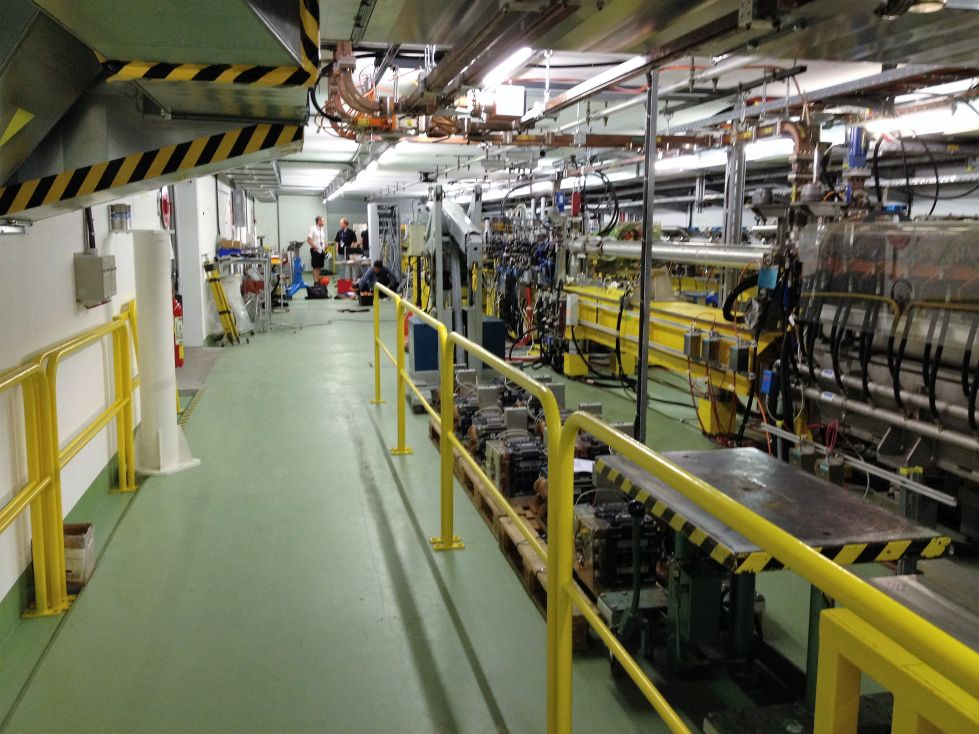
\includegraphics[width=\linewidth]{images/CLIC-CTF3-overview}
    \end{subfigure}
	\hfill
    \begin{subfigure}{0.47\linewidth}
		\centering
		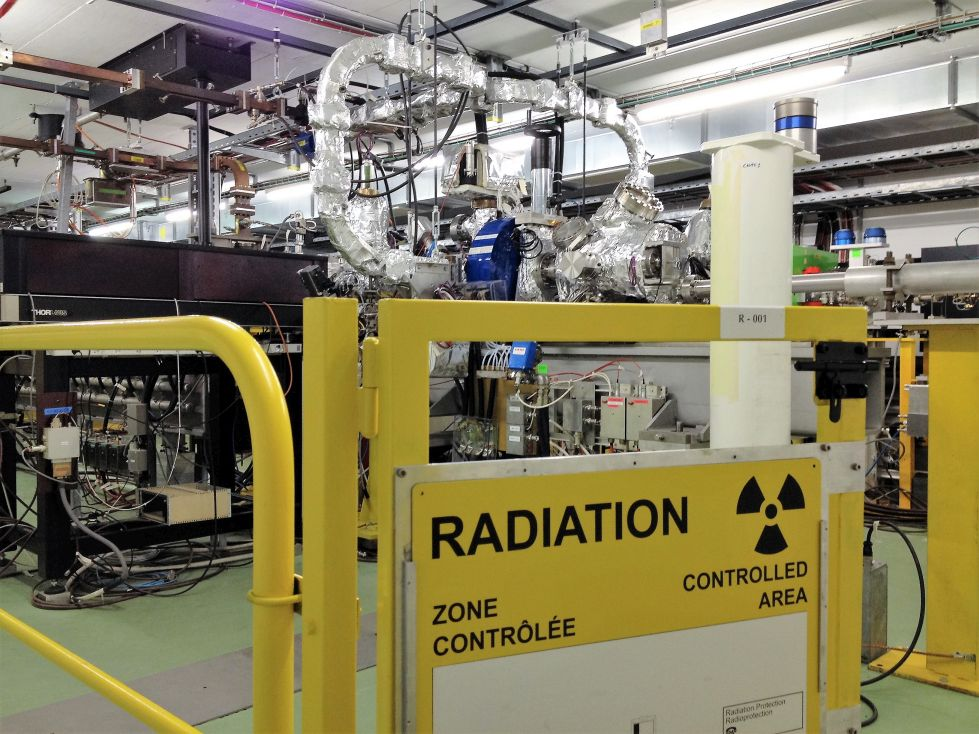
\includegraphics[width=\linewidth]{images/CLIC-CTF3-radiation}
    \end{subfigure}
	\par\bigskip
    \begin{subfigure}{0.47\linewidth}
		\centering
		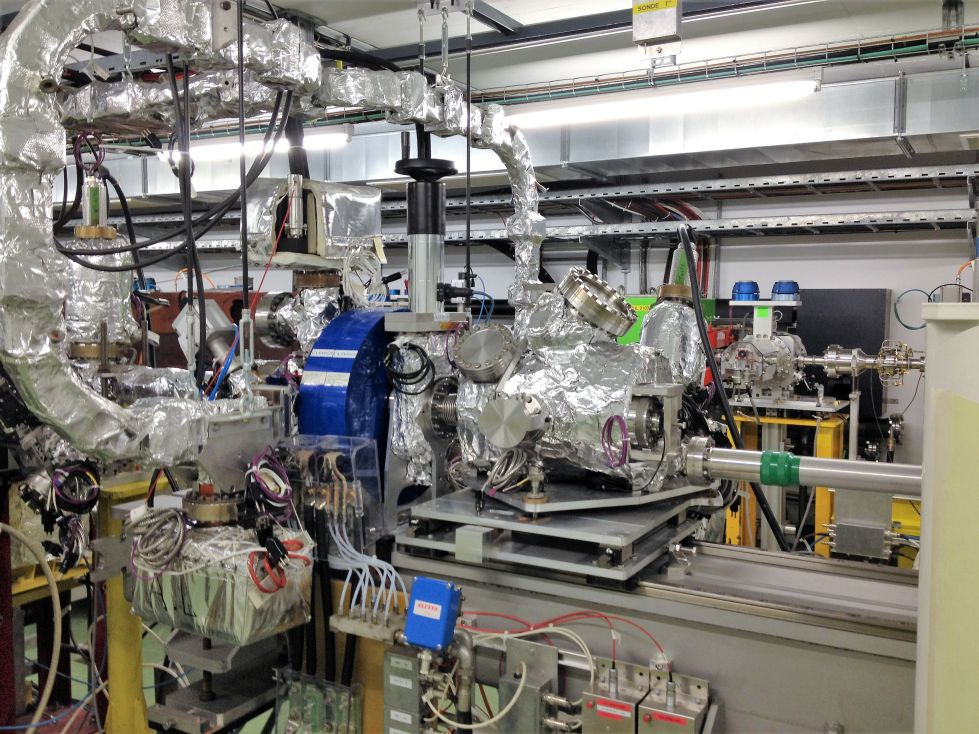
\includegraphics[width=\linewidth]{images/CLIC-CTF3-img1}
    \end{subfigure}        
	\hfill
    \begin{subfigure}{0.47\linewidth}
		\centering
		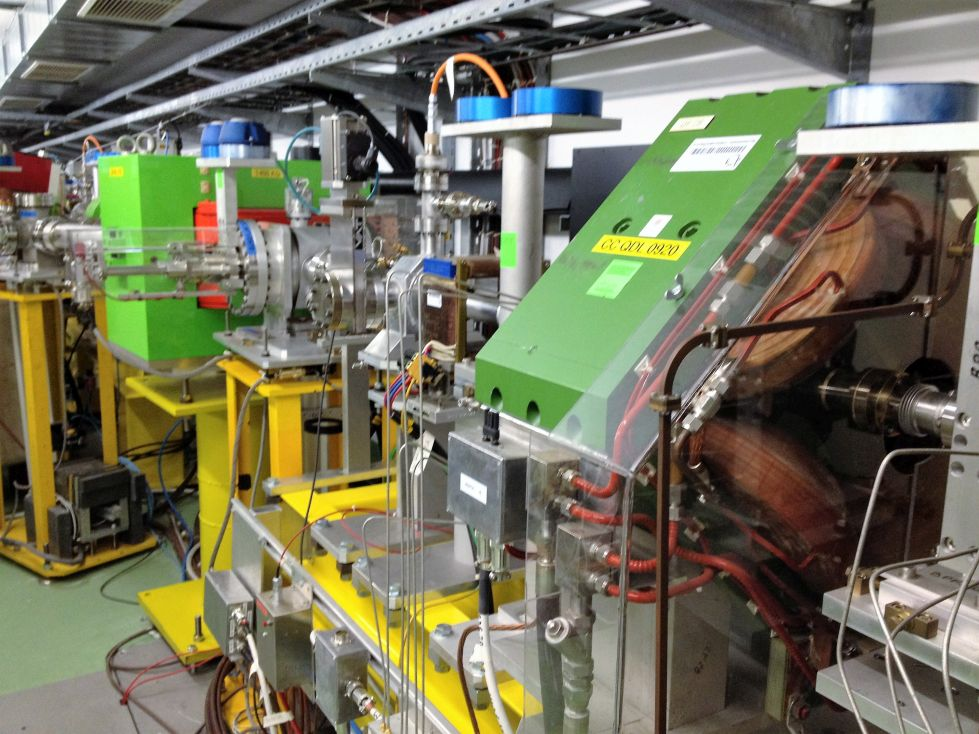
\includegraphics[width=\linewidth]{images/CLIC-CTF3-img2}
    \end{subfigure}
	\par\bigskip
    \begin{subfigure}{0.47\linewidth}
		\centering
		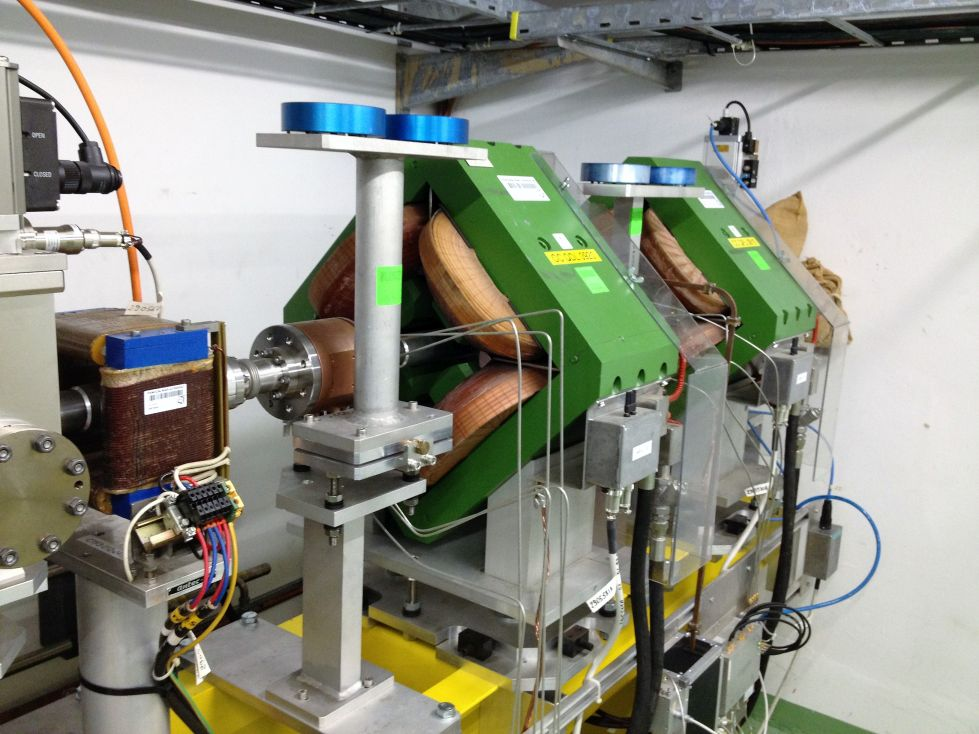
\includegraphics[width=\linewidth]{images/CLIC-CTF3-img3}
    \end{subfigure}        
	\hfill
    \begin{subfigure}{0.47\linewidth}
		\centering
		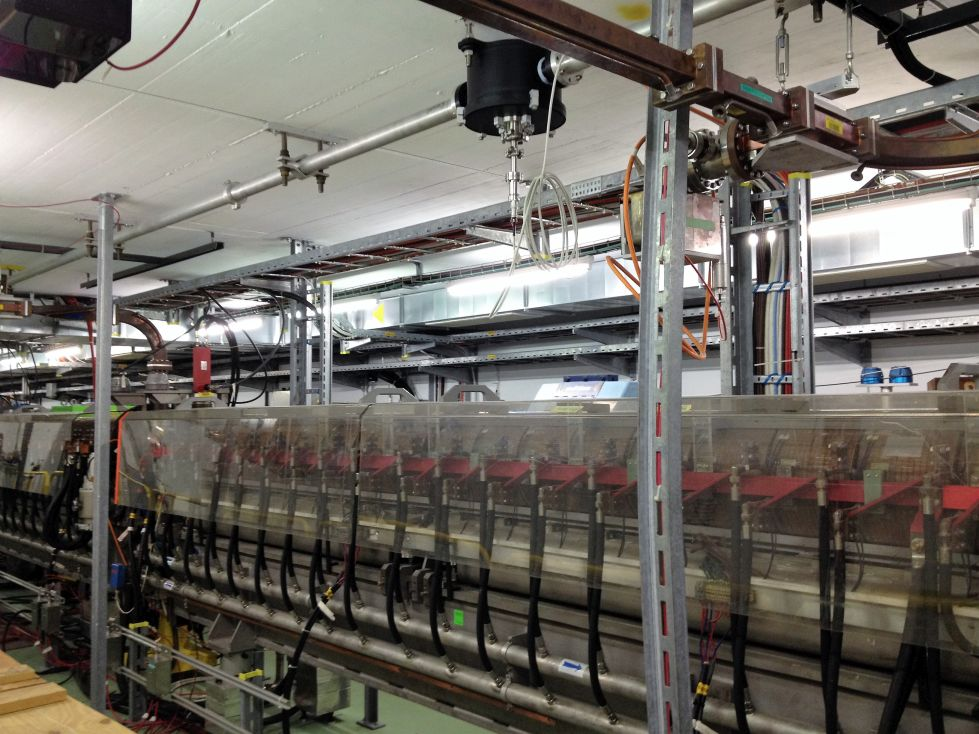
\includegraphics[width=\linewidth]{images/CLIC-CTF3-img4}
    \end{subfigure}
\caption[Εικόνες από το \en{CLIC Testing Facility 3}]
{Εικόνες από το \en{CLIC Testing Facility 3 (CTF3)}, όπου γίνονται δοκιμές για το \en{CLIC}. 
Λόγω της φύσης των δοκιμών, το \en{CTF3} θεωρείται \en{$``$radiation controlled zone$"$} και για την είσοδο κάποιου στο χώρο απαιτείται να έχει περάσει 7-ωρη εκπαίδευση (\en{radiation training}) και να φέρει ειδικό δοσίμετρο κατά την επίσκεψη}
\label{img:CLIC-CTF3}        
\end{figure}



\section{\selectlanguage{greek}Ο \en{Electron Beam Scanner}}

\subsection{Εισαγωγή}

Όπως αναφέρεται και προηγουμένως, ο \en{CLIC} αποσκοπεί σε επιτάχυνση των \SI[per-mode = symbol]{100}{\mega \volt \per \metre} και χρησιμοποιεί την καινοτομία των δύο δεσμών για να πετύχει αυτό το στόχο. 
Ως εκ τούτου, είναι απαραίτητο η Δέσμη Οδηγός (\en{Drive Beam}) να έχει πολύ μεγάλη ένταση, το οποίο καθιστά πρόκληση τη μέτρηση της χωρικής έντασης (προφίλ) της δέσμης αυτής. 
Επεμβατικές μέθοδοι, όπως για παράδειγμα το \en{wire scanner}, χρησιμοποιούνται ευρέως σε επιταχυντές. Όμως λόγω της έντασης της δέσμης θα καταστρέφονταν. 
Έτσι οδηγούμαστε στην αναζήτηση νέων μη επεμβατικών μεθόδων για την κάλυψη αυτού του κενού.

Μια μη επεμβατική μέθοδος που εξετάζεται είναι η μέθοδος του \en{Electron Beam Scanner}, όπου μια δέσμη ανίχνευσης (\en{probe beam}) στέλνεται κάθετα προς τη Δέσμη Οδηγό (\en{Drive Beam}). 
Ανιχνεύοντας τη δέσμη ανίχνευσης και μετρώντας την εκτροπή της σε σχέση με την αρχική της θέση, είναι εφικτός ο υπολογισμός του προφίλ της Δέσμης Οδηγού.

Ανιχνευτές \en{Electron Beam Scanner} έχουν χρησιμοποιηθεί στο παρελθόν σε άλλους επιταχυντές που έχουν συνεχείς και πολύ μακριές δέσμες, όπου η κατανομή του φορτίου θεωρείται σταθερή κατά τη μέτρηση.
Η Δέσμη Οδηγός του \en{CLIC} θα έχει δέσμες μήκους μόλις \num{12} \en{picoseconds}. 
Αυτό δημιουργεί πρόσθετες προκλήσεις για τη λειτουργία του \en{Electron Beam Scanner}.
Στην παρούσα εργασία θα εξετάσουμε τη λειτουργία ενός \en{Electron Beam Scanner} σε επιταχυντή που το μήκος της δέσμης είναι σημαντικά μικρότερο από το χρόνο σάρωσης της δέσμης ανίχνευσης. 
Συγκεκριμένα, η περίπτωση όπου το μήκος της δέσμης είναι μικρότερο από το χρόνο που απαιτείται για ένα σωματίδιο της δέσμης ανίχνευσης να διασχίσει τη κύρια δέσμη είναι δύσκολο να μοντελοποιηθεί αναλυτικά. 
Δημιουργήθηκε για αυτό το σκοπό ένα περιβάλλον προσομοίωσης για να προσομοιωθεί αυτή η κατάσταση.

\subsection{Σχετική βιβλιογραφία} %TODO find a better title 
Ακολουθώντας την αρχική έρευνα από τους \en{Pasour} και \en{Ngo} \cite{Pasour1992}, ανιχνευτές \en{Electron Beam Scanner} έχουν χρησιμοποιηθεί επιτυχώς για την μέτρηση του εγκάρσιου προφίλ δέσμης σε διάφορους επιταχυντές, όπως τον δακτύλιο \en{Spallation Neutron Source (SNS)} στο \en{Oak Ridge National Laboratory} \cite{Aleksandrov2005} \cite{Blokland2009} και τη δέσμη \en{NTX} στο \en{Lawrence Berkeley National Laboratory} \cite{Roy2005}. 
Αυτοί οι επιταχυντές έχουν μεγάλο μήκος δέσμης εκατοντάδων \en{nanoseconds}. 
Έτσι, η εγκάρσια κατανομή φορτίου μπορεί να θεωρηθεί σταθερή κατά τη μέτρηση.

Ο \en{Electron Beam Scanner} δουλεύει μετρώντας την εκτροπή της δέσμης ανίχνευσης που αποτελείται από χαμηλής ενέργειας ηλεκτρόνια, καθώς αυτά διαπερνούν κάθετα την κύρια δέσμη (Σχήμα \ref{fig:beam-deflection}).
Για την απεικόνιση επιλέξαμε σε αυτή τη διπλωματική εργασία ότι μετράμε το εγκάρσιο προφίλ, και ότι η δέσμη οδηγός ταξιδεύει οριζοντίως. 
Φυσικά, το προφίλ μπορεί να μετρηθεί σε κάθε άξονα στρέφοντας τη διάταξη. 


\begin{figure}[tph]
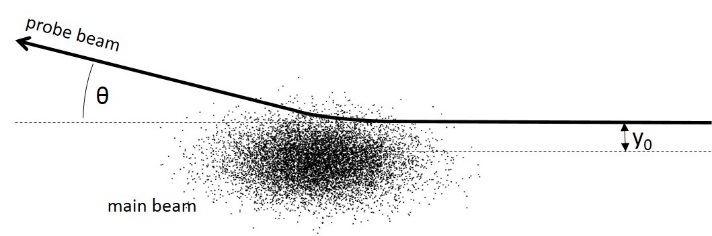
\includegraphics[width=0.8\linewidth]{figures/Beam-deflection}
\centering
\caption{Εκτροπή δέσμης ανίχνευσης από την μετρούμενη δέσμη}
\label{fig:beam-deflection}
\end{figure}

Η γωνία απόκλισης $\theta$ της δέσμης οδηγού μετράται για διαφορετικές τιμές ύψους $y_0$, και το προφίλ της κύριας δέσμης $\delta (y)$ είναι ανάλογο του διαφορικού  \cite{Blokland2009}

\begin{equation} \label{eq:transverseProfile}
\frac{\dd{} |\theta|}{\dd y_0} \propto \delta (y)
\end{equation}

Η σταθερά αναλογίας εξαρτάται από την ενέργεια της δέσμης ανίχνευσης. 
Εδώ έχουν γίνει οι εξής απλοποιητικές υποθέσεις:
\begin{enumerate}
\item Η απόκλιση είναι μικρή
\item Η μεταβολή ενέργειας της δέσμης ανίχνευσης είναι αμελητέα 
\item Η επίδραση του μαγνητικού πεδίου της κύριας δέσμης είναι πολύ μικρότερη από αυτή του ηλεκτρικού πεδίου
\end{enumerate} 

Για να μετρηθεί η γωνία απόκλισης για διαφορετικά $y_0$ σε μία εικόνα, σαρώνεται διαγώνια η αρχική θέση της δέσμης οδηγού. 

Ένας \en{Electron Beam Scanner} έχει επίσης χρησιμοποιηθεί στο \en{Budker Institute for Nuclear Physics} για τη μέτρηση πολύ κοντύτερων δεσμών στον επιταχυντή \en{VEPP-5} \cite{Logatchov2006}, με μήκος δέσμης της τάξης μεγέθους του \SI{1}{\nano \second}.
Σε αυτή την περίπτωση η εγκάρσια κατανομή φορτίου μεταβάλλεται κατά τη μέτρηση.
Έτσι, όχι μόνο η απόκλιση της δέσμης στην κάθετη διεύθυνση δεν είναι σταθερή, αλλά υπάρχει και πρόσθετη απόκλιση κατά μήκος του άξονα της δέσμης του επιταχυντή, λόγω του κατά μήκος διαφορικού του φορτίου.

Σε τέτοιες περιπτώσεις, μια (μη σαρωμένη) δέσμη ανίχνευσης αποκλίνει έτσι, ώστε το ίχνος να αφήνει μια έλλειψη στην οθόνη κάθε φορά που περνά μια δέσμη.
Ο λόγος των αξόνων της έλλειψης καθορίζεται από το μήκος της δέσμης και το φορτίο.
Ολόκληρο το διαμήκες προφίλ μπορεί να υπολογιστεί μετρώντας την ένταση της δέσμης ανίχνευσης γύρω από την έλλειψη \cite{Logatchov1999}.
Μετρώντας έναν αριθμό ελλείψεων με διαφορετικές αρχικές θέσεις, λαμβάνοντας τη μέγιστη απόκλιση κάθε έλλειψης και εφαρμόζοντας τη σχέση \ref{eq:transverseProfile} δίνεται το εγκάρσιο προφίλ.
Έτσι μπορούμε να μετρήσουμε το διαμήκες και το εγκάρσιο προφίλ με μία μόνο συσκευή.

Στην παρούσα διπλωματική εργασία θα εξετάσουμε τη λειτουργία ενός \en{Electron Beam Scanner} σε επιταχυντή που το μήκος της δέσμης είναι σημαντικά μικρότερο από το χρόνο σάρωσης της δέσμης ανίχνευσης. 
Συγκεκριμένα, η περίπτωση όπου το μήκος της δέσμης είναι μικρότερο από το χρόνο που απαιτείται για ένα σωματίδιο της δέσμης ανίχνευσης να διασχίσει τη κύρια δέσμη είναι δύσκολο να μοντελοποιηθεί αναλυτικά. 
Η πλήρωση αυτής της συνθήκης εξαρτάται από διάφορους παράγοντες, όπως την ενέργεια της δέσμης ανίχνευσης και το μέγεθος της μετρούμενης δέσμης, αλλά μπορεί να ειπωθεί κατά προσέγγιση ότι εφαρμόζεται σε δέσμες με μήκος μικρότερο των \SI{100}{\pico \second}.

Ένα παράδειγμα τέτοιας δέσμης είναι ο προτεινόμενος επιταχυντής \en{Compact LInear Collider (CLIC)}. 
Η δέσμη οδηγός του \en{CLIC} θα επιταχύνει μια δέσμη ηλεκτρονίων υψηλής έντασης έως τα \SI{2.4}{\giga \electronvolt} \cite{Aicheler2012}.
Ο επιταχυντής της δέσμης οδηγού θα είναι γραμμικός επιταχυντής των \SI{1}{\giga \hertz}.
Θα εισάγεται σε εναλλασσόμενα δοχεία, δίνοντας κενό μεταξύ των δεσμών (\en{bunch spacing}) \SI{2}{\nano \second}.
Στο τέλος του γραμμικού επιταχυντή, θα χρησιμοποιείται ένα σύστημα πολλαπλασιασμού συχνότητας \cite{Biscari2009} για να μειώσει το κενό μεταξύ των δεσμών στα \SI{0.083}{\nano \second}, πολλαπλασιάζοντας έτσι το ρεύμα κατά \num{24} και μειώνοντας το μήκος του παλμού κατά τον ίδιο συντελεστή.
Έπειτα, η ενέργεια της δέσμης οδηγού θα μεταφέρεται στην κύρια δέσμη με τη χρήση ειδικά σχεδιασμένων συζευγμένων κοιλοτήτων που επιτρέπουν την επιτάχυνση με ρυθμό που φτάνει πάνω από \SI[per-mode = symbol]{100}{\mega \volt \per \meter} \cite{Degiovanni2014}.

\begin{table}[tph]
\centering
	\begin{tabular}{l c}
		\hline
		\en{Bunch population}	& \SI{5e10}{\electrons} \\ \hline
		\en{Transverse Emittance}	& \SI{100}{\nano \meter \radian} \\\hline
		\en{Bunch length / spacing}	& \SI{13}{\pico \second} / \SI{2}{\nano \second} \\\hline
		\en{Pulse length}	& \SI{140}{\micro \second} \\\hline
		\en{Pulse Population}		& \SI{3e15}{\electrons} \\\hline
		\en{Repetition Frequency}	& \SI{50}{\Hz} \\\hline
	\end{tabular}
\caption[Σχετικές παράμετροι για την Δέσμη Οδηγό του επιταχυντή \en{CLIC}]{Σχετικές παράμετροι για την Δέσμη Οδηγό του επιταχυντή \en{CLIC} \protect{\cite{Aicheler2012}}}
\label{tab:parameters}
\end{table}

Το εγκάρσιο προφίλ της δέσμης θα πρέπει να μετράται σε διάφορα σημεία κατά μήκος του γραμμικού επιταχυντή, και μη επεμβατικοί μετρητές προφίλ αναπτύσσονται για αυτό το σκοπό.
Οι μετρητές πρέπει να έχουν ανάλυση \SI{100}{\micro \meter} ή καλύτερη, ώστε να μετράει το ελάχιστο μέγεθος ακτίνας κατά τη διάρκεια \en{quad scans}.
Επεμβατικές μέθοδοι, όπως οθόνες \en{OTR (Optical Transition Radiation)} μπορούν να εγκατασταθούν παράλληλα για βαθμονόμηση, αλλά για χρήση μόνο κατά τη διάρκεια της λειτουργίας με μειωμένο μήκος παλμών.

\subsection{Θεωρητική ανάλυση του \en{Electron Beam Scanner}} \label{sub:EBS-model}
Η λεπτή δέσμη ανίχνευσης κινείται κατά τον άξονα $X$, είναι κάθετη στην κίνηση της σχετικιστικής κίνησης της κύριας δέσμης (άξονας $Z$), με παράμετρο απόκλισης $\rho$ (Σχήμα \ref{fig:ellipse-EBS}).

\begin{figure}[tph]
	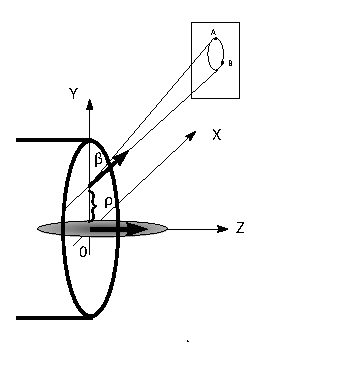
\includegraphics[width=0.6\linewidth]{figures/Logatchov1999-EBS}
	\centering
	\caption{Διαδικασία ανίχνευσης της χαρακτηριστικής έλλειψης της δέσμης}
	\label{fig:ellipse-EBS}
\end{figure}

Τα αποτελέσματα της σάρωσης λαμβάνονται σε οθόνη παράλληλη στο επίπεδο $Y-Z$ και σε απόσταση $L$ από τον άξονα $Z$.

Έστω ότι το κέντρο της κύριας δέσμης βρίσκεται στην αρχή των αξόνων τη χρονική στιγμή $t = 0$, ενώ η δέσμη ανίχνευσης έχει ομοιόμορφη πυκνότητα κατά $X$ και διάμετρο $d \ll \rho$.
Εδώ υποθέτουμε ότι το $\rho$ είναι μεγαλύτερο του τυπικού εγκάρσιου μεγέθους της κύριας δέσμης.
Τη χρονική στιγμή $t = 0$ κάθε  σωματίδιο της δέσμης ανίχνευσης αντιστοιχίζεται σε μια συγκεκριμένη θέση $x$.
Η συνολική γωνία απόκλισης κατά $Y$ για κάθε σωματίδιο υπό την επιρροή του ηλεκτρικού πεδίου της κύριας δέσμης μπορεί να εκφραστεί ως\cite{Logatchov1999}:
\begin{equation}
\theta_y (x) = \frac{2 \rho r_e}{\beta} \int_{-\infty}^{\infty}\frac{n(z) \dd z}{\rho^2 + \left(x+\beta z \right) ^2}
\end{equation}
όπου:
\begin{itemize}
\item $r_e$: η κλασική ακτίνα του ηλεκτρονίου,
\item $\beta =\frac{v_t}{c}$: η σχετική ταχύτητα της δέσμης ανίχνευσης,
\item $c$: η ταχύτητα του φωτός,
\item $x$: η θέση σωματιδίου της δέσμης ανίχνευσης τη χρονική στιμή $t=0$,
\item $n(z)$: η γραμμική πυκνότητα της κύριας δέσμης κατά τον άξονα $Z$.
\end{itemize} 

Η έκφραση για τη γωνία απόκλισης του σωματιδίου κατά $Z$, λόγω του μαγνητικού πεδίου, μπορεί να γραφεί\cite{Logatchov1999}:
\begin{equation}
\theta_z(x) = 2 r_e \int_{-\infty}^{\infty}\frac{(x+\beta z)n(z) \dd z}{\rho^2 + \left(x+\beta z \right) ^2}
\end{equation}
\chapter{Μέθοδοι προσομοίωσης}
Στο κεφάλαιο αυτό περιγράφεται η υλοποίηση του συστήματος, με βάση τη μελέτη που παρουσιάστηκε στο προηγούμενο κεφάλαιο. 
Αρχικά παρουσιάζεται η πλατφόρμα και τα προγραμματιστικά εργαλεία που χρησιμοποιήθηκαν. 

\section{Εργαλεία που χρησιμοποιήθηκαν}
Για την υλοποίηση των προσομοιώσεων χρησιμοποιήθηκε το πρόγραμμα \en{CST Particle Studio}, της σουίτας προγραμμάτων προσομοίωσης \en{CST Studio Suite}. 
Για την επεξεργασία των αποτελεσμάτων χρησιμοποιήθηκε το πρόγραμμα \en{MATLAB}. 
Τα προγράμματα παρουσιάζονται πιο αναλυτικά παρακάτω.

\subsection{Το \en{CST Particle Studio}}
\begin{figure}[tph]

\includegraphics[width=0.25\textwidth]{images/CST-logo.png}
\centering
\caption{Το λογότυπο του \en{CST}}
\label{img:CSTlogo}
\end{figure}
Το \en{CST PARTICLE STUDIO\textsuperscript{\textregistered} (CST\textsuperscript{\textregistered} PS) } είναι ένα εξειδικευμένο εργαλείο για την γρήγορη και ακριβή ανάλυση δυναμικών φορτισμένων σωματιδίων σε τρισδιάστατα ηλεκτρομαγνητικά πεδία.
Είναι ένα ισχυρό εργαλείο, κατάλληλο για μεγάλο φάσμα εργασιών, από σχεδιασμό \en{magnetrons} και ρύθμιση σωλήνων ηλεκτρονίως έως μοντελοποίηση πηγών σωματιδίων και εξαρτημάτων για επιταχυντές.

%\en{The particle tracking solver can model the behavior of particles through static fields, and with the gun iteration, space charge limited emission. 
Ο \en{particle-in-cell (PIC) solver}, ο οποίος μπορεί να λειτουργήσει στο πεδίο του χρόνου, μπορεί να εκτελέσει μια πλήρη προσομοίωση σωματιδίων και ηλεκτρομαγνητικών πεδίων.

Για σχετικιστικές εφαρμογής, ο \en{wakefield solver} μπορεί να υπολογίσει πώς τα πεδία που δημιουργούνται από σωματίδια που κινούνται στην (ή κοντά στην) ταχύτητα του φωτός, αλληλεπιδρούν με τη δομή γύρω τους.

Το \en{CST PS} έχει ενσωματωμένα τα \en{3D EM modules} του \en{CST STUDIO SUITE\textsuperscript{\textregistered}}, όπως τα \en{CST EM STUDIO\textsuperscript{\textregistered} electro- and magnetostatic solvers} και το \en{CST MICROWAVE STUDIO\textsuperscript{\textregistered} eigenmode solver}.

Είναι πλήρως ενσωματωμένα στο περιβάλλον σχεδίασης \en{CST STUDIO SUITE}, χρησιμοποιώντας έτσι τις δυνατότητες μοντελοποίησης και τα \en{import interfaces}.

Το \en{CST PS} βασίζεται στη γνώση, την έρευνα και την ανάπτυξη των αλγορίθμων που χρησιμοποιήθηκαν στο πακέτο προσομοίωσης \en{MAFIA-4}. 
Ο \en{PIC solver} μπορεί επίσης να εκμεταλλευτεί δυνατότητες \en{GPU computing}, προσφέροντας σημαντικές βελτιώσεις στην απόδοση, σε συμβατό υλικό.

\subsection{Το \en{MATLAB}}
Το \en{MATLAB (matrix laboratory)} είναι ένα περιβάλλον αριθμητικής υπολογιστικής και μια προγραμματιστική γλώσσα τέταρτης γενιάς. 
\en{A proprietary programming language developed by MathWorks, MATLAB allows matrix manipulations, plotting of functions and data, implementation of algorithms, creation of user interfaces, and interfacing with programs written in other languages, including C, C\nolinebreak\hspace{-.05em}\raisebox{.4ex}{\tiny\bf +}\nolinebreak\hspace{-.10em}\raisebox{.4ex}{\tiny\bf +}, C$\sharp$, Java, Fortran and Python.}

\en{Although MATLAB is intended primarily for numerical computing, an optional toolbox uses the MuPAD symbolic engine, allowing access to symbolic computing abilities. 
An additional package, Simulink, adds graphical multi-domain simulation and model-based design for dynamic and embedded systems.}

\begin{figure}[tph]

\includegraphics[width=0.25\textwidth]{images/Matlab-logo.png}
\centering
\caption{Το λογότυπο του \en{MATLAB}}
\label{img:MATLABlogo}
\end{figure}

\section{Επιρροή διάφορων μεταβλητών σε έναν \en{Electron Beam Scanner}}
\subsection{Θεωρητική βάση}
Η λεπτή δέσμη ανίχνευσης κινείται κατά τον άξονα $X$, είναι κάθετη στην κίνηση της σχετικιστικής κίνησης της κύριας δέσμης (άξονας $Z$), με παράμετρο απόκλισης $\rho$ (Σχήμα \ref{fig:ellipse-EBS}).

\begin{figure}[tph]
	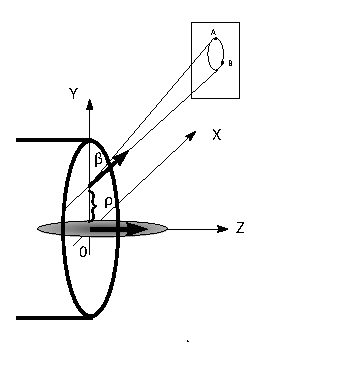
\includegraphics{figures/Logatchov1999-EBS}
	\centering
	\caption{Διαδικασία ανίχνευσης της χαρακτηριστικής έλλειψης της δέσμης}
	\label{fig:ellipse-EBS}
\end{figure}

Τα αποτελέσματα της σάρωσης γίνονται \en{monitor} σε οθόνη παράλληλη στο επίπεδο $Y-Z$ και σε απόσταση $L$ από τον άξονα $Z$.

Έστω ότι το κέντρο της κύριας δέσμης βρίσκεται στην αρχή των αξόνων τη χρονική στιγμή $t = 0$, ενώ η δέσμη ανίχνευσης έχει ομοιόμορφη πυκνότητα κατά $X$ και διάμετρο $d \ll \rho$.
Εδώ υποθέτουμε ότι το $\rho$ είναι μεγαλύτερο του τυπικού εγκάρσιου μεγέθους της κύριας δέσμης.
Τη χρονική στιγμή $t = 0$ κάθε  σωματίδιο της δέσμης ανίχνευσης αντιστοιχίζεται σε μια συγκεκριμένη θέση $x$.
Η συνολική γωνία απόκλισης κατά $Y$ για κάθε σωματίδιο υπό την επιρροή του ηλεκτρικού πεδίου της κύριας δέσμης μπορεί να εκφραστεί ως\cite{Logatchov1999}:
\begin{equation}
\theta_y (x) = \frac{2 \rho r_e}{\beta} \int_{-\infty}^{\infty}\frac{n(z) \dd z}{\rho^2 + \left(x+\beta z \right) ^2}
\end{equation}
όπου:
\begin{itemize}
\item $r_e$: η κλασσική ακτίνα του ηλεκτρονίου,
\item $\beta =\frac{v_t}{c}$: η σχετική ταχύτητα της δέσμης ανίχνευσης,
\item $c$: η ταχύτητα του φωτός,
\item $x$: η θέση σωματιδίου της δέσμης ανίχνευσης τη χρονική στιμή $t=0$,
\item $n(z)$: η γραμμική πυκνότητα της κύριας δέσμης κατά τον άξονα $Z$.
\end{itemize} 

Η έκφραση για τη γωνία απόκλισης του σωματιδίου κατά $Z$, λόγω του μαγνητικού πεδίου, μπορεί να γραφεί\cite{Logatchov1999}:
\begin{equation}
\theta_z(x) = 2 r_e \int_{-\infty}^{\infty}\frac{(x+\beta z)n(z) \dd z}{\rho^2 + \left(x+\beta z \right) ^2}
\end{equation}
\subsection{Αποτελέσματα ανάλυσης με το \en{MATLAB}}
Ιδιαίτερο ενδιαφέρον για την έναρξη της ανάλυσής μας παρουσιάζει το πώς διάφορες μεταβλητές επηρεάζουν τα στοιχεία της χαρακτηριστικής έλλειψης. 
Συγκεκριμένα, θα διερευνήσουμε πώς επηρεάζουν τη χαρακτηριστική έλλειψη οι:
\begin{enumerate}
	\item Ένταση της δέσμης ανίχνευσης
	\item Μήκος της δέσμης ανίχνευσης
	\item Αρχική θέση ριπής κατά $Y$ ($\rho$) 
	\item Τάση της δέσμης ανίχνευσης
\end{enumerate}

Για τη διερεύνηση αυτή δημιουργήθηκε ένα \en{script} στο \en{MATLAB}, όπου χρησιμοποιήθηκε το μοντέλο που παρουσιάστηκε προηγουμένως και έγιναν οι μελέτες για το πώς επηρεάζει η κάθε παράμετρος ξεχωριστά. 
Τα αποτελέσματα φαίνονται παρακάτω.

\begin{figure}[tph]	
	\begin{subfigure}{0.45\textwidth}
		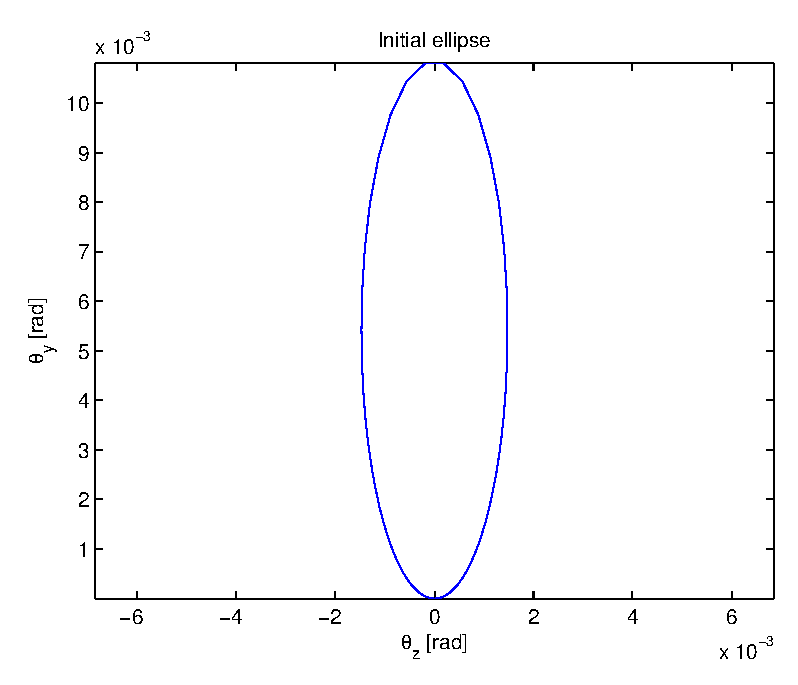
\includegraphics[width=0.9\linewidth]{figures/beam-deflection-script-01-initial-elipse}
		\centering
		\caption{Η χαρακτηριστική έλλειψη στην αρχική κατάσταση}
		\label{fig:beam-deflection-script-01-initial-elipse}
	\end{subfigure}
	~
	\begin{subfigure}{0.45\textwidth}
		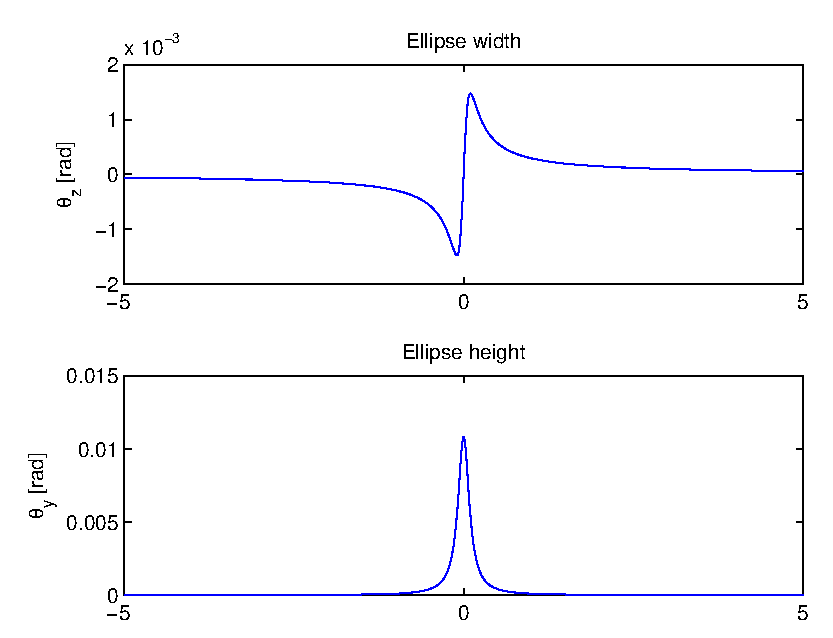
\includegraphics[width=0.9\linewidth]{figures/beam-deflection-script-02-elipse-width}
		\centering
		\caption{Το πλάτος και ύψος της έλλειψης στην αρχική κατάσταση}
		\label{fig:beam-deflection-script-02-elipse-width}
	\end{subfigure}
\caption{Απεικόνιση και στοιχεία της χαρακτηριστικής έλλειψης στην αρχική κατάσταση}
\label{fig:initial-ellipse}
\end{figure}

\begin{figure}[tph]	
	\begin{subfigure}{0.45\textwidth}
		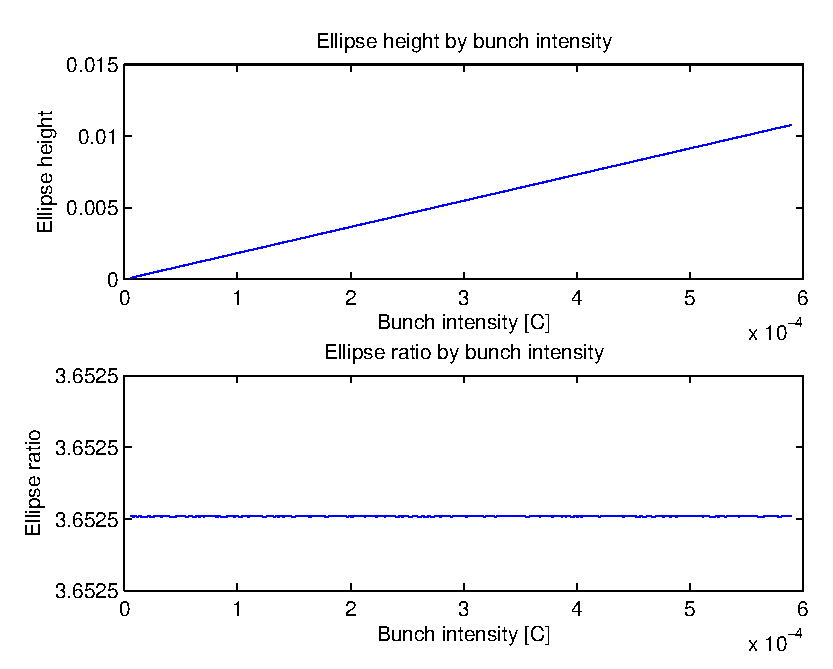
\includegraphics[width=0.9\linewidth]{figures/beam-deflection-script-03-elipse-height}
		\centering
		\caption{Επιρροή της έντασης της δέσμης ανίχνευσης στην ύψος και το λόγο της έλλειψης}
		\label{fig:beam-deflection-script-03-elipse-height}
	\end{subfigure}
	~
	\begin{subfigure}{0.45\textwidth}
		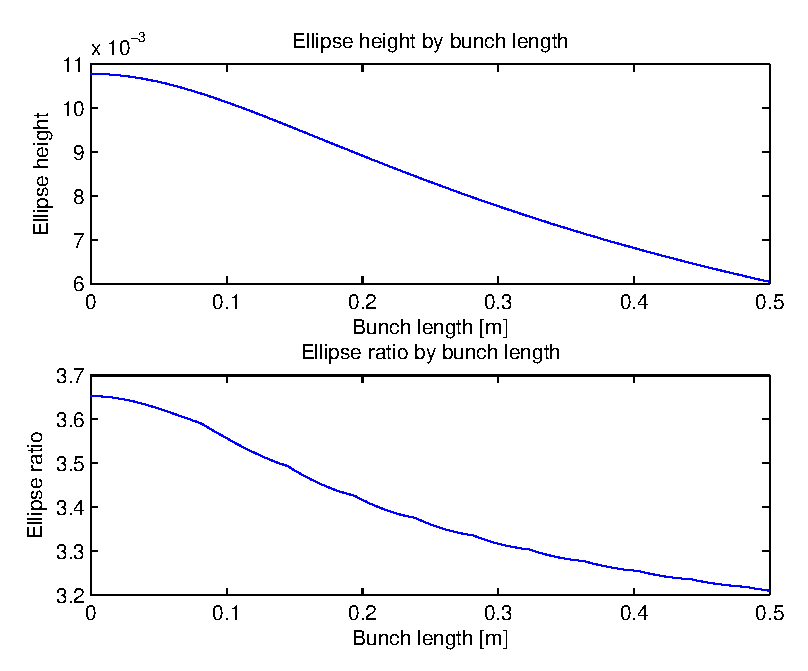
\includegraphics[width=0.9\linewidth]{figures/beam-deflection-script-04-elipse-height-by-bunch-intensity}
		\centering
		\caption{Επιρροή του μήκους της δέσμης ανίχνευσης στην ύψος και το λόγο της έλλειψης}
		\label{fig:beam-deflection-script-04-elipse-height-by-bunch-intensity}
	\end{subfigure}
	\par\bigskip
	\begin{subfigure}{0.45\textwidth}
		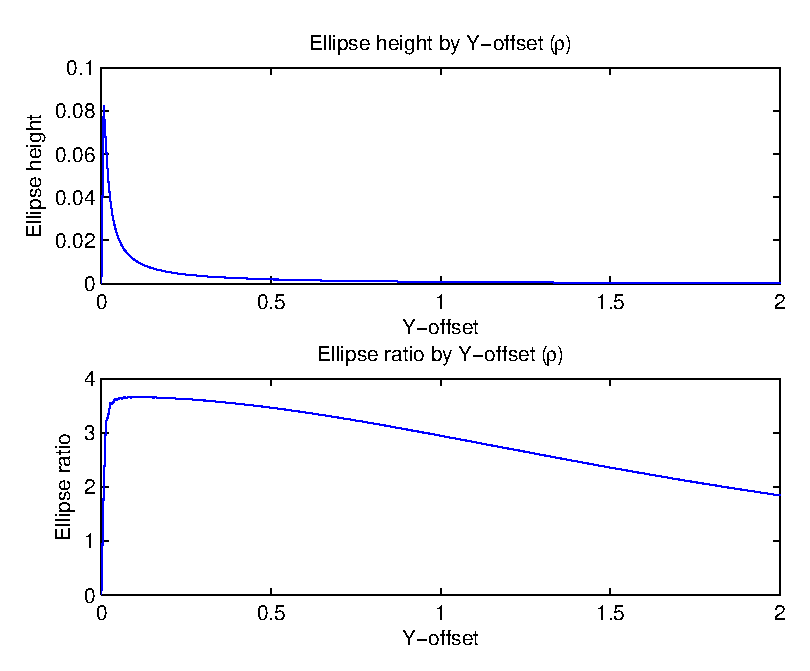
\includegraphics[width=0.9\linewidth]{figures/beam-deflection-script-05-elipse-ratio-by-bunch-intensity}
		\centering
		\caption[Επιρροή της αρχικής θέσης ριπής της δέσμης ανίχνευσης στην ύψος και το λόγο της έλλειψης]{Επιρροή της αρχικής θέσης ριπής ($Y$-\en{offset}) της δέσμης ανίχνευσης στην ύψος και το λόγο της έλλειψης}
		\label{fig:beam-deflection-script-05-elipse-ratio-by-bunch-intensity}
	\end{subfigure}
	~
	\begin{subfigure}{0.45\textwidth}
		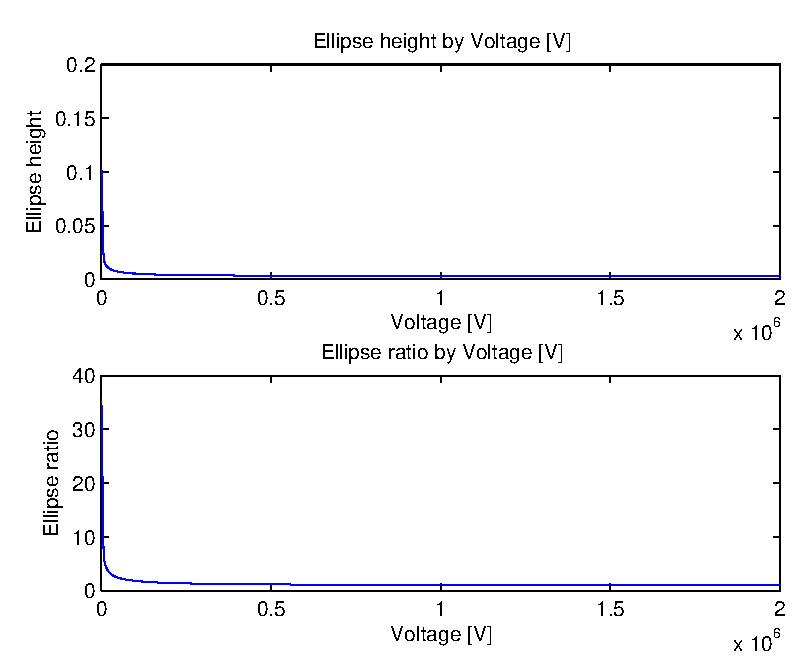
\includegraphics[width=0.9\linewidth]{figures/beam-deflection-script-06}
		\centering
		\caption{Επιρροή της γραμμικής μεταβολής τάσης της δέσμης ανίχνευσης στην ύψος και το λόγο της έλλειψης}
		\label{fig:beam-deflection-script-06}
	\end{subfigure}
	\par\bigskip
	\begin{subfigure}{0.45\textwidth}
		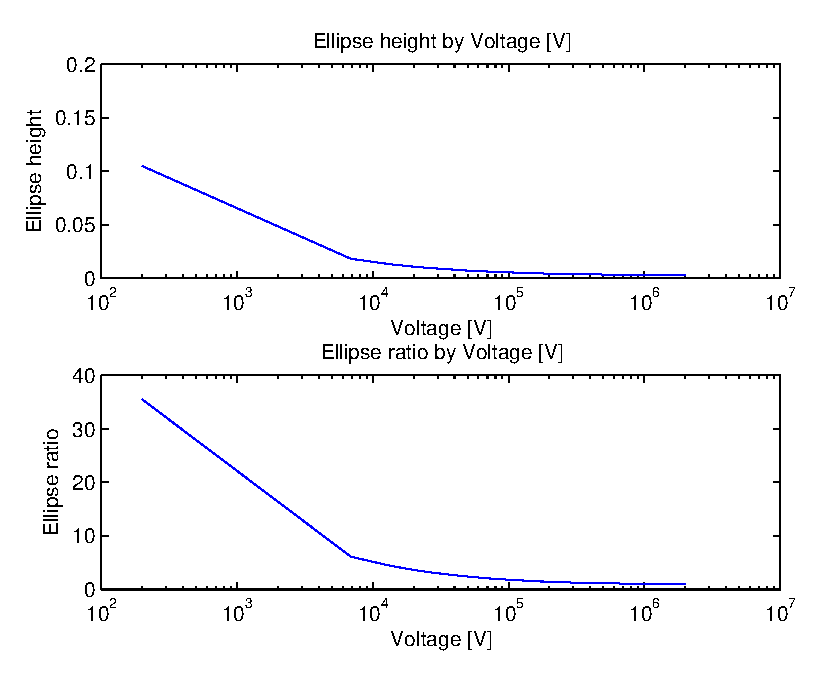
\includegraphics[width=0.9\linewidth]{figures/beam-deflection-script-07}
		\centering
		\caption{Επιρροή της εκθετικής μεταβολής τάσης της δέσμης ανίχνευσης στην ύψος και το λόγο της έλλειψης}
		\label{fig:beam-deflection-script-07}
	\end{subfigure}
\caption{Επιρροή διαφόρων μεγεθών στη χαρακτηριστική έλλειψη}
\label{fig:beam-deflectoin}
\end{figure}

\subsection{Αποτελέσματα ανάλυσης με το \en{CST}}

Στη συνέχεια έγινε η ίδια ανάλυση στο περιβάλλον προσομοίωσης του \en{CST} για την επαλήθευση των αποτελεσμάτων. 
Για να γίνει αυτό αρχικά δημιουργήθηκε το περιβάλλον προσομοίωσης, και σε αυτό μπήκαν οι  δυο κύλινδροι, μέσα στους οποίους βρίσκονται οι 2 δέσμες, η κύρια δέσμη και η δέσμη ανίχνευσης (Σχήμα \ref{fig:CST-PICmonitor}). 
Στη συνέχεια προστέθηκαν οι πηγές σωματιδίων ως κυκλικές πηγές, με την κύρια πηγή να έχει \en{Gaussian} προφίλ, ενώ η πηγή της δέσμης ανίχνευσης σταθερό. 
Η πηγή σωματιδίων της κύριας δέσμης φαίνεται στο Σχήμα \ref{fig:CST-mainBeamSource}.

\begin{figure}[tbh]
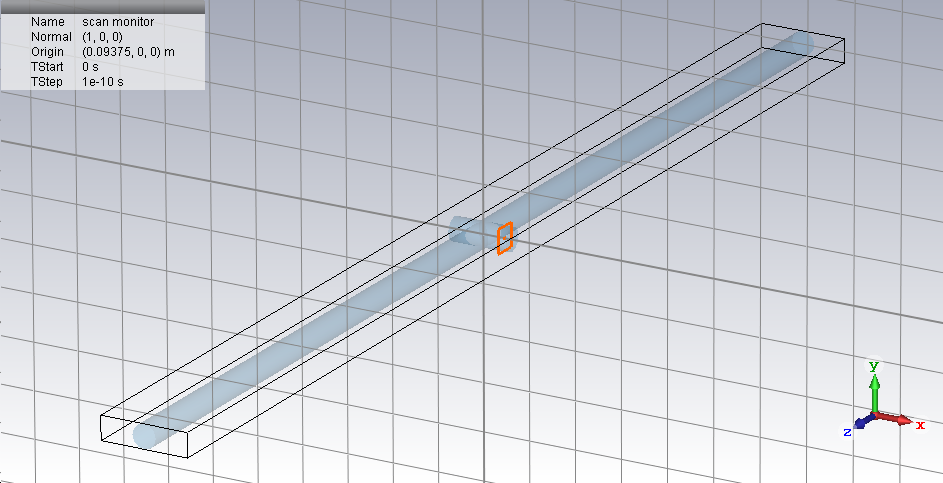
\includegraphics[width=\textwidth]{figures/CST-pic-monitor}
\centering
\caption[Η διάταξη προσομοιωμένη στο \en{CST}]{Η διάταξη προσομοιωμένη στο \en{CST}. 
Στην κύρια δέσμη φαίνεται ανιχνευτής σωματιδίων λίγο πριν το σημείο που γίνεται η ανίχνευση}
\label{fig:CST-PICmonitor}
\end{figure}

\begin{figure}[tbh]
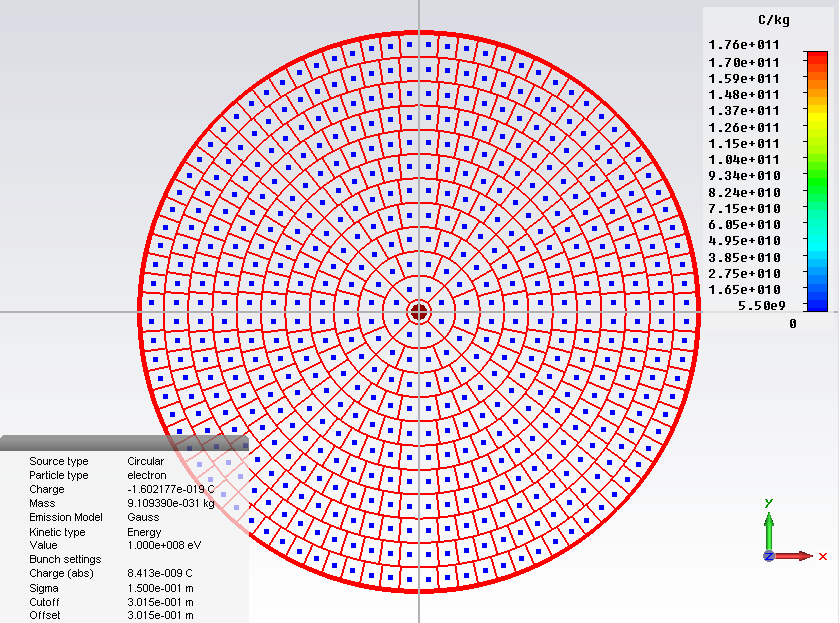
\includegraphics[width=0.5\textwidth]{figures/CST-main-beam-source}
\centering
\caption{Η πηγή της κύριας δέσμης στο \en{CST}}
\label{fig:CST-mainBeamSource}
\end{figure}

Τα αποτελέσματα της προσομοίωσης σε φαίνονται παρακάτω. 

%TODO create and add images of the simulation (file 0.21?)

\section{Εκτίμηση του προφίλ στατικής δέσμης στο \en{CST}}

Αφού είδαμε ότι είναι εφικτό να μετρηθούν τα χαρακτηριστικά με τον τρόπο που προσομοιώνει το \en{CST}, ως επόμενο βήμα θα υπολογίσουμε το ακριβές προφίλ της δέσμης, δηλαδή θα δημιουργήσουμε έναν \en{Electron Beam Scanner}.

\begin{figure}[tph]
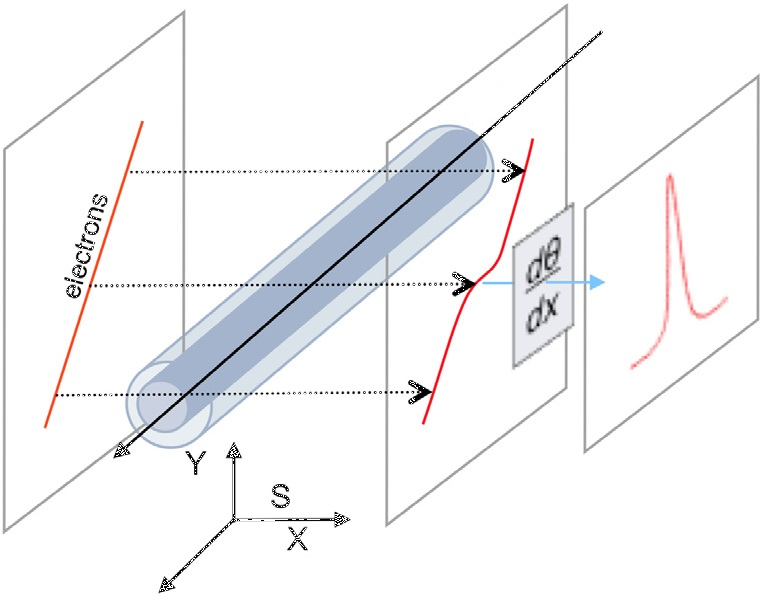
\includegraphics[width=0.5\textwidth]{figures/EBS-profile-calculation}
\centering
\caption{Υπολογισμός του προφίλ δέσμης με \en{Electron Beam Scanner}}
\label{fig:EBS-profile-calculation}
\end{figure}

Όπως είδαμε και στο προηγούμενο κεφάλαιο, το προφίλ της δέσμης προκύπτει από την παραγώγιση  της απόκλισης $\theta_y$.

Στην περίπτωσή μας, ο υπολογισμός τους προφίλ γίνεται μέσα στο \en{CST}, στο στάδιο του \en{post-processing}.



\section{Εκτίμηση του προφίλ \en{Gaussian} δέσμης στο \en{CST}}

Για τον υπολογισμό του προφίλ μιας \en{Gaussian} δέσμης, συναντήσαμε το πρόβλημα ότι μετά τον υπολογισμό του προφίλ, το σχήμα δε φαινόταν να έχει αυτό που ήταν αναμενόμενο.

\begin{figure}[tph]
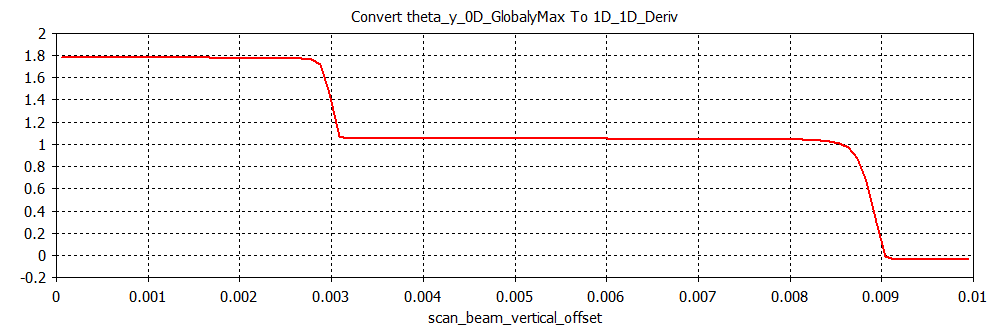
\includegraphics[width=\textwidth]{figures/CST-profile-steps}
\centering
\caption{Το αποτέλεσμα του υπολογισμού του προφίλ στο \en{CST} δε μοιάζει \en{Gaussian}}
\label{fig:CST-profile-steps}
\end{figure}

Για την επίλυση του προβλήματος αυτού, αρχικά ελέγξαμε αν το πρόβλημα βρίσκεται στον τρόπο δημιουργίας της δέσμης ή στον τρόπο ανίχνευσης. 
Έτσι:
\begin{enumerate}
\item Δημιουργήσαμε ένα νέο project και, αφού στήθηκε όλο το μοντέλο εκ νέου, μπήκε ένας \en{particle monitor} που ανιχνεύει τα σωματίδια της κύριας δέσμης
\item Έγινε εξαγωγή των δεδομένων αυτών της κύριας δέσμης
\item Τα δεδομένα αυτά εισήχθησαν στο \en{MATLAB} και δημιουργήθηκε το κατάλληλο \en{script} για την ανάλυσή τους
\end{enumerate}

Από την παραπάνω διαδικασία έγινε σαφές ότι το πρόβλημα εντοπίζεται στον τρόπο που το \en{CST} δημιουργεί την κατανομή των σωματιδίων.

\subsection{Τρόπος δημιουργίας \en{Gaussian} κατανομών σωματιδίων στο \en{CST}}

Μετά από αναζήτηση και επικοινωνία με το ίδιο το \en{support} του \en{CST}, έγινε σαφής ο τρόπος που γίνεται η προσομοίωση των σωματιδίων για \en{Gaussian} κυκλικές πηγές σωματιδίων.
%TODO citation needed
Συγκεκριμένα, αρχικά, αφού το συνολικό ποσό φορτίου που εκπέμπεται δεν μεταβάλλεται ανάλογα με τη συνάρτηση κατανομής τίθεται ο περιορισμός ότι:
\begin{equation}\label{eq:CST-gaussian-restriction}
2\pi \int_{R_{in}}^{R_{out}} f(r) \dd r = \pi \left(R_{out}^2 - R_{in}^2 \right) 
\end{equation}

όπου:
\begin{itemize}
\item $R_{out}$: η εξωτερική ακτίνα της κυκλικής πηγής σωματιδίων
\item $R_{in}$: η εσωτερική ακτίνα της κυκλικής πηγής σωματιδίων (στην περίπτωσή μας $R_{in} = 0$)
\item $f(r)$: η συνάρτηση ακτινικής κατανομής 
\end{itemize} 

Η παραπάνω σχέση χρησιμοποιείται για να κλιμακοποιήσει τη συνάρτηση κατανομής. 
Αυτό σημαίνει ότι ο συντελεστής κατανομής $c_{scale}$ υπολογίζεται αυτόματα.

Στη συνέχεια, η \en{Gaussian} κατανομή δίνεται από τη σχέση:
\begin{equation}
f(r) = c_{off} + c_{scale} \left( \exp \left(-\frac{r^2}{2\sigma^2}\right) - 1 \right)
\end{equation}

όπου:
\begin{itemize}
\item $c_{off}$: η τιμή της συνάρτησης για $r = 0$
\item $\sigma$: η τυπική απόκλιση
\end{itemize} 

\begin{figure}[tph]
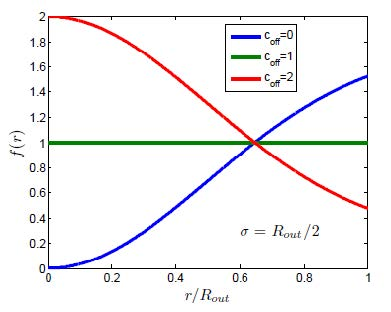
\includegraphics{figures/CST-gauss-function-for-coff}
\centering
\caption{Παράδειγμα \en{Gaussian} συνάρτησης για διάφορες τιμές του συντελεστή $c_{off}$}
\label{fig:CST-gauss-coff}
\end{figure}

Για να έχουμε μια πραγματικά \en{Gaussian} δέσμη, θέλουμε να ισχύει
\[c_{off} = 0\]

Αφού οι υπόλοιπες μεταβλητές είναι καθορισμένες από τις απαιτήσεις του επιταχυντή, απομένει να βρεθεί η τιμή του $c_{scale}$ που θα μας δίνει τη ζητούμενη συνθήκη.

\subsection{Υπολογισμός του κατάλληλου συντελεστή κλιμακοποίησης για \en{Gaussian} δέσμη}

Ο τρόπος που υπολογίζει το \en{CST} την \en{Gaussian} κατανομή, όπως είδαμε παραπάνω είναι
\begin{eqnarray}\label{eq:CST-gaussian-model}
f(r) &= & 	c_{off} + c_{scale} \left( \exp \left(-\frac{r^2}{2\sigma^2}\right) - 1 \right) \nonumber \\
&= &\left(c_{off} - c_{scale}\right) + c_{scale} e^{-\frac{r^2}{2\sigma^2}}
\end{eqnarray}

Η πραγματική κατανομή της δέσμης στον επιταχυντή που μελετούμε όμως, έχει γενική μορφή κατανομής:
\begin{equation}\label{eq:General-gaussian-model}
 f(r) = a e^{-\frac{\left(r-b\right)^2}{2c^2}}
\end{equation}

Επομένως, εξισώνοντας τις παραπάνω σχέσεις \ref{eq:CST-gaussian-model} και \ref{eq:General-gaussian-model} και δεδομένου ότι πρέπει να ισχύουν $\forall r$ προκύπτουν τα συμπεράσματα ότι:
\begin{eqnarray}
a &\equiv & c_{scale}\nonumber \\
b &\equiv &0\nonumber \\
c &\equiv & \sigma \nonumber \\
c_{off} &=&  c_{scale} 
\end{eqnarray}

Επομένως, πρέπει να βρεθεί ο κατάλληλος συνδυασμός τιμών $\left(c_{off}, c_{scale}\right)$ που να πληροί τον περιορισμό της εξίσωσης \ref{eq:CST-gaussian-restriction}, δεδομένων των τιμών των μεταβλητών $\sigma, R_{out}$ και $R_{in}$ του επιταχυντή μας.

Για την επίλυση του παραπάνω προβλήματος δημιουργήθηκε κατάλληλο \en{script} στο \en{MATLAB}. 

Αρχικά δημιουργήθηκε η συνάρτηση \src{c-scale = calculate-cscale( sigma, c-off, Rout, Rin)} η οποία δέχεται ως ορίσματα τις μεταβλητές $\sigma, c_{off}, R_{out}$ και $R_{in}$ και δίνει στην έξοδό του την τιμή του $c_{scale}$ που πληροί την εξίσωση \ref{eq:CST-gaussian-restriction}.

Στη συνέχεια, τρέχοντας το \en{script} \src{find-optimum-coff.m} δίνουμε τις τιμές των παραμέτρων του προβλήματός μας στα $\sigma, c_{off}, R_{out}, R_{in}$ και βρίσκουμε την τιμή του $c_{off}$ που επαληθεύει τη σχέση $c_{off} = c_{scale} \left(\sigma, c_{off}, R_{out}, R_{in} \right)$.

\lstinputlisting[caption={\tg{Η συνάρτηση υπολογισμού του $c_{scale}$}}]{code/Calculating-optimum-coff/calculate-cscale.m}
\lstinputlisting[caption={\tg{Το }\en{script}\tg{ υπολογισμού του κατάλληλου για τα δεδομένα μας $c_{off}$}}]{code/Calculating-optimum-coff/find-optimum-coff.m}
%TODO fix this shit

Εν τέλει, για τις τιμές του δικού μας προβλήματος, δίνουμε ως είσοδο $\left(\sigma, R_{out}, R_{in} \right) = \left(0.01/4,0.01, 0 \right)$ και προκύπτει ότι:
\begin{equation}
c_{off} \approx 8.002684
\end{equation}

\section{Επιρροή αλλεπάλληλων δεσμών στο προφίλ δέσμης}

\section{Επαλήθευση αποτελεσμάτων στο \en{MATLAB}}


\chapter{Αποτελέσματα}
% Some examples illustrating the dependence on bunch intensity, bunch length and transverse size, plus at least on example from the multi-bunch simulations.


\section{Επίδραση παραμέτρων του επιταχυντή στην ανίχνευση της δέσμης}

\subsection{Αποτελέσματα θεωρητικού μοντέλου}
Τα αποτελέσματα της ανάλυσης που παρουσιάστηκε στην υπο-ενότητα \ref{sub:variable-analysis-MATLAB} φαίνονται παρακάτω.

\begin{figure}[tph]	
	\begin{subfigure}{0.47\textwidth}
		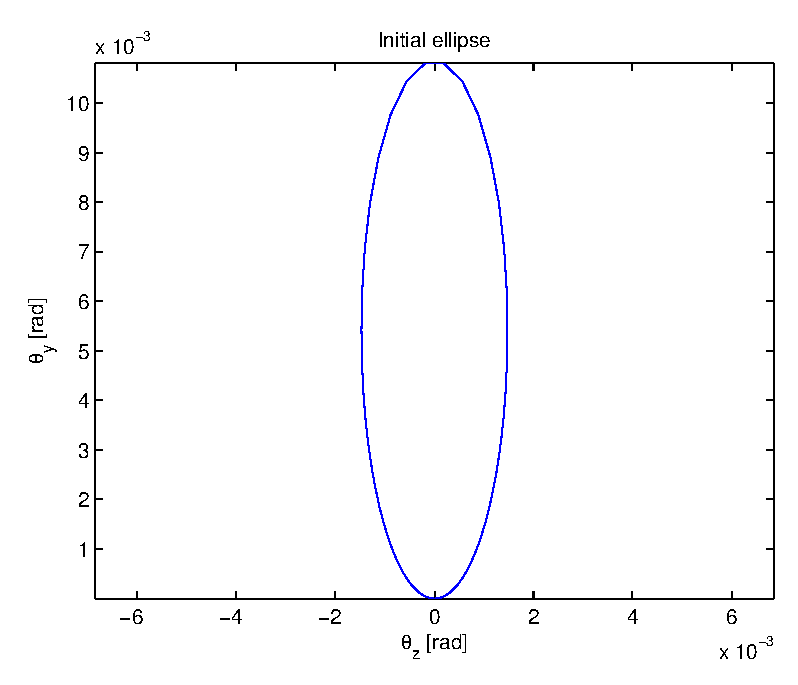
\includegraphics[width=\linewidth]{figures/beam-deflection-script-01-initial-elipse}
		\centering
		\caption{Η χαρακτηριστική έλλειψη στην αρχική κατάσταση}
		\label{fig:beam-deflection-script-01-initial-elipse}
	\end{subfigure}
	\hfill
	\begin{subfigure}{0.47\textwidth}
		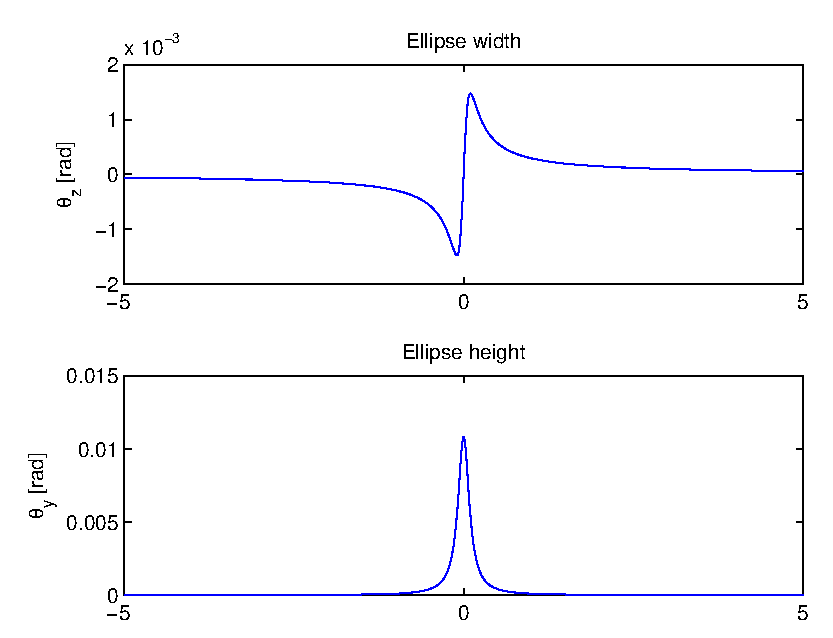
\includegraphics[width=\linewidth]{figures/beam-deflection-script-02-elipse-width}
		\centering
		\caption{Το πλάτος και ύψος της έλλειψης στην αρχική κατάσταση}
		\label{fig:beam-deflection-script-02-elipse-width}
	\end{subfigure}
\caption{Απεικόνιση και στοιχεία της χαρακτηριστικής έλλειψης στην αρχική κατάσταση}
\label{fig:initial-ellipse}
\end{figure}

\begin{figure}[tph]	
	\begin{subfigure}{0.47\textwidth}
		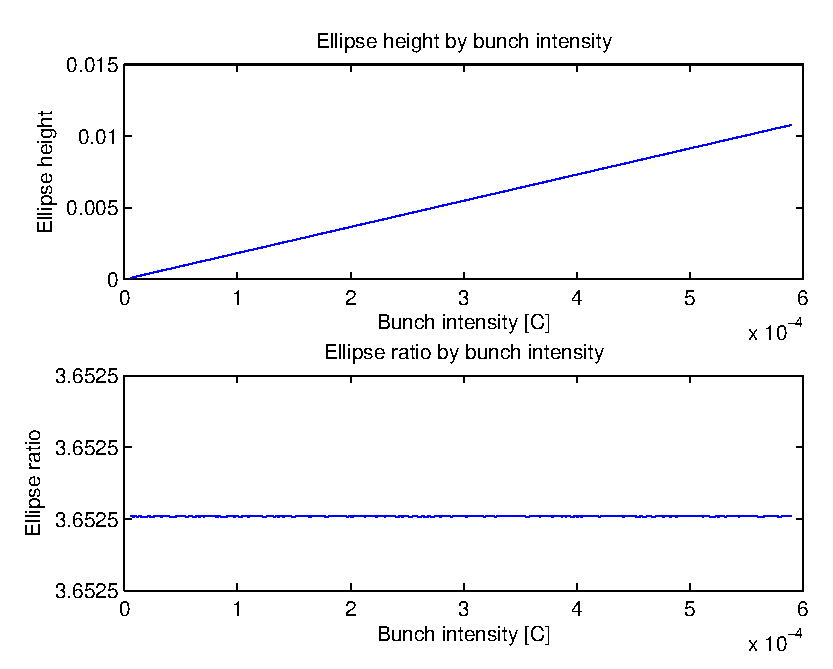
\includegraphics[width=\linewidth]{figures/beam-deflection-script-03-elipse-height}
		\centering
		\caption{Επιρροή της έντασης της δέσμης ανίχνευσης στην ύψος και το λόγο της έλλειψης}
		\label{fig:beam-deflection-script-03-elipse-height}
	\end{subfigure}
	\hfill
	\begin{subfigure}{0.47\textwidth}
		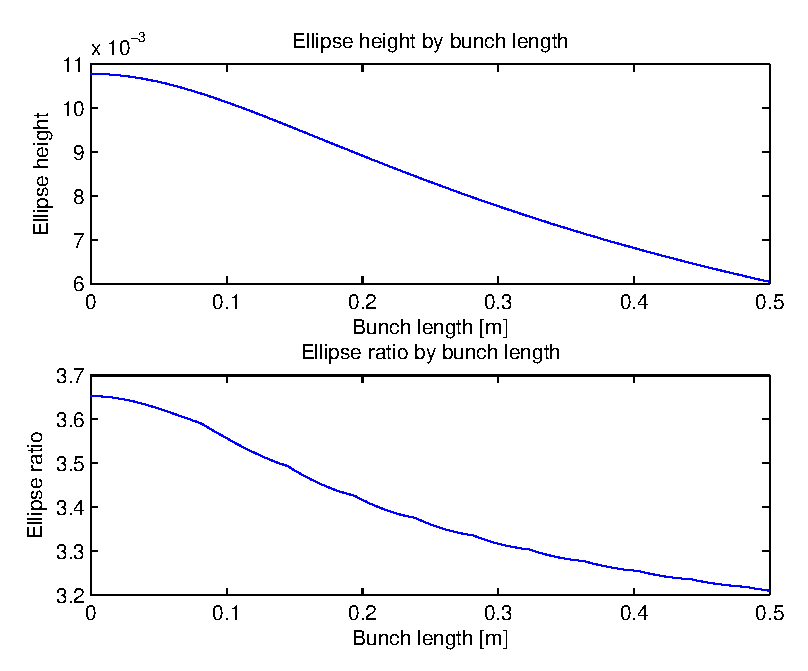
\includegraphics[width=\linewidth]{figures/beam-deflection-script-04-elipse-height-by-bunch-intensity}
		\centering
		\caption{Επιρροή του μήκους της δέσμης ανίχνευσης στην ύψος και το λόγο της έλλειψης}
		\label{fig:beam-deflection-script-04-elipse-height-by-bunch-intensity}
	\end{subfigure}
	\par\bigskip
	\begin{subfigure}{0.47\textwidth}
		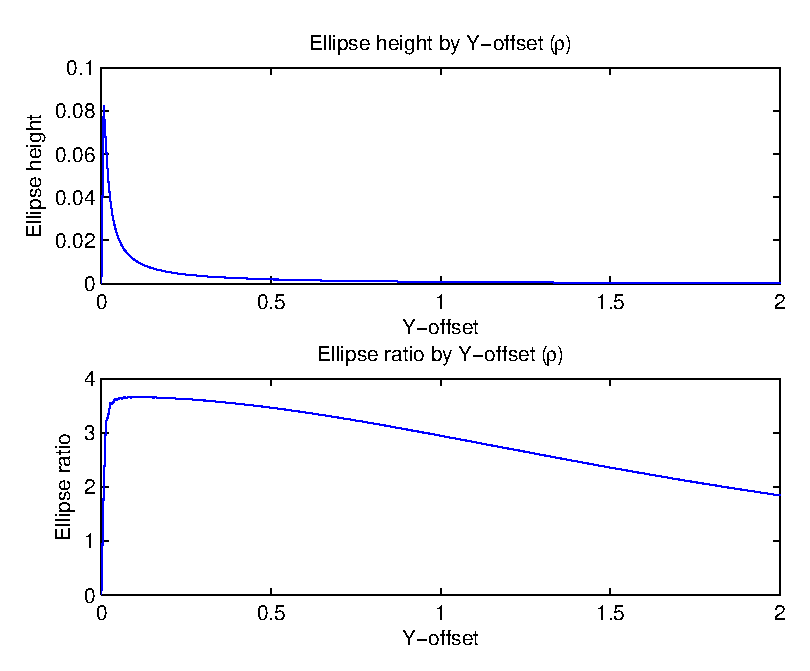
\includegraphics[width=\linewidth]{figures/beam-deflection-script-05-elipse-ratio-by-bunch-intensity}
		\centering
		\caption[Επιρροή της αρχικής θέσης ριπής της δέσμης ανίχνευσης στην ύψος και το λόγο της έλλειψης]{Επιρροή της αρχικής θέσης ριπής ($Y$-\en{offset}) της δέσμης ανίχνευσης στην ύψος και το λόγο της έλλειψης}
		\label{fig:beam-deflection-script-05-elipse-ratio-by-bunch-intensity}
	\end{subfigure}
	\hfill
	\begin{subfigure}{0.47\textwidth}
		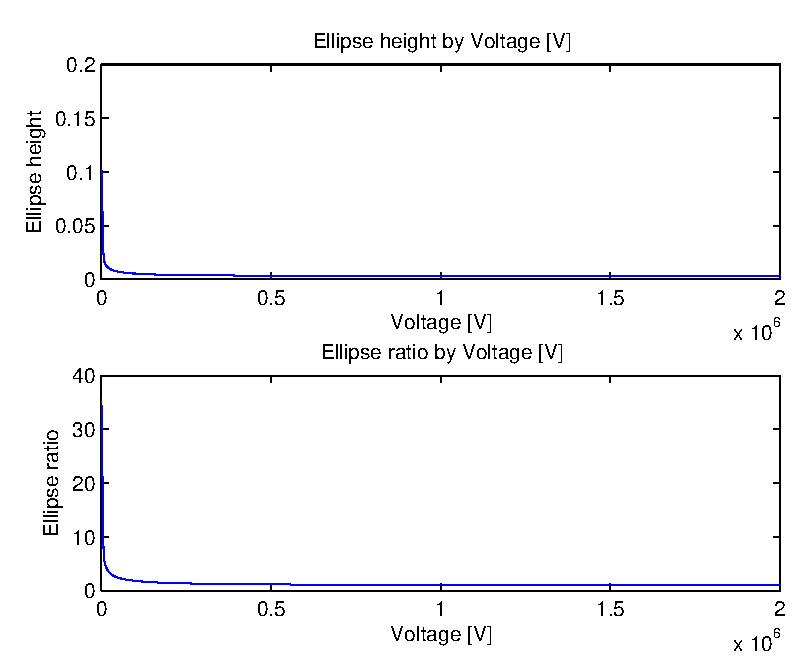
\includegraphics[width=\linewidth]{figures/beam-deflection-script-06}
		\centering
		\caption{Επιρροή της γραμμικής μεταβολής τάσης της δέσμης ανίχνευσης στην ύψος και το λόγο της έλλειψης}
		\label{fig:beam-deflection-script-06}
	\end{subfigure}
	\par\bigskip
	\begin{subfigure}{0.47\textwidth}
		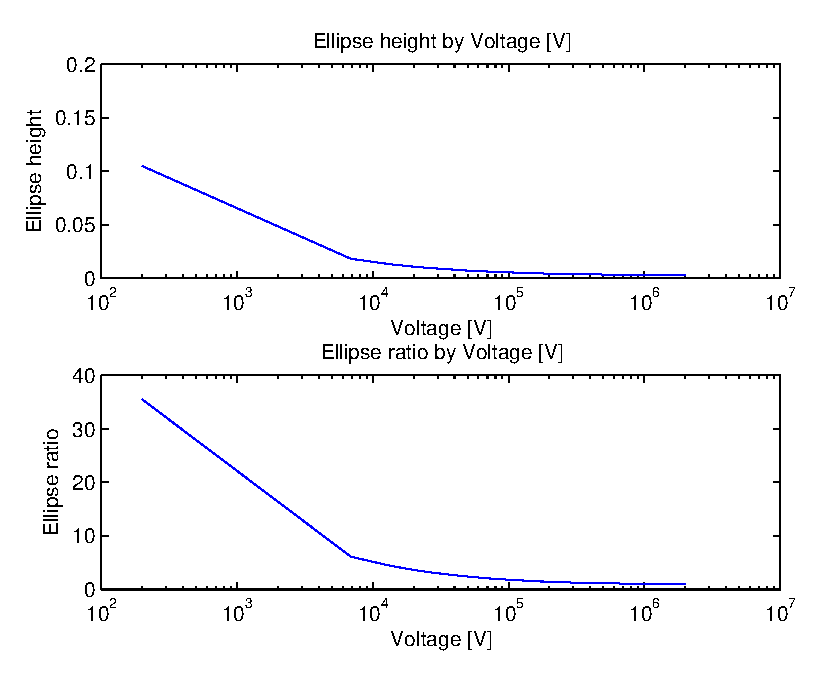
\includegraphics[width=\linewidth]{figures/beam-deflection-script-07}
		\centering
		\caption{Επιρροή της εκθετικής μεταβολής τάσης της δέσμης ανίχνευσης στην ύψος και το λόγο της έλλειψης}
		\label{fig:beam-deflection-script-07}
	\end{subfigure}
\caption{Επιρροή διαφόρων μεγεθών στη χαρακτηριστική έλλειψη}
\label{fig:beam-deflectoin}
\end{figure}

\subsection{Αποτελέσματα προσομοίωσης}

\subsection{Σύγκριση αποτελεσμάτων}

\section{Αποτελέσματα προσομοίωσης της μεθόδου στο \en{CST}}


\section{Αποτελέσματα ανάλυσης με χρήση \en{CST} και \en{MATLAB}}





\chapter{Επίλογος}
Σε αυτό το τελευταίο παρουσιάζονται κάποια συμπεράσματα που μπορούν να εξαχθούν από τη διπλωματική εργασία, καθώς και ενδεχόμενες μελλοντικές επεκτάσεις όσων παρουσιάστηκαν.

\section{Συμπεράσματα}
Τα συμπεράσματα που προέκυψαν από τη διπλωματική είναι τα παρακάτω:
\begin{itemize}
\item Το \en{CST} είναι ένα εργαλείο που μπορεί να αντεπεξέλθει αποτελεσματικά στις ανάγκες της έρευνας στην κατεύθυνση εναλλακτικών τρόπων σάρωσης του προφίλ δεσμών ηλεκτρονίων, με χρήση του εξαιρετικά ισχυρού \en{CST Particle Studio} και του \en{particle-in-cell (PIC) solver}.
\item Για πολλαπλές επαναλαμβανόμενες προσομοιώσεις όπου το \en{CST} θα πρέπει να υπολογίζει ίδιες τροχιές, καθίσταται μη αποδοτικό λόγω περιορισμών του προγράμματος στο να χαρακτηρίζονται τμήματα της προσομοίωσης ως $``$όχι απαραίτητα για υπολογισμό εκ νέου σε κάθε προσομοίωση$"$. 
Για τέτοιες περιπτώσεις η επιστράτευση εργαλείων όπως το \en{MATLAB} διευκολύνει την απόδοση και αυξάνει την ελευθερία διαχείρισης των αποτελεσμάτων στον χρήστη τους.
\item Ο \en{Electron Beam Scanner} αποτελεί έναν τρόπο ανίχνευσης του εγκάρσιου προφίλ δέσμης σωματιδίων ο οποίος, μετά από μια αρχική ανάλυση, φαίνεται να είναι ένας από τους πολλά υποσχόμενους τρόπους μη επεμβατικής ανίχνευσης.
\end{itemize}

\section{Μελλοντικές Επεκτάσεις}
Το σύστημα που αναπτύχθηκε στα πλαίσια αυτής της διπλωματικής εργασίας θα μπορούσε να βελτιωθεί και να επεκταθεί περαιτέρω,
τουλάχιστον ως προς τρεις κατευθύνσεις. 
Συγκεκριμένα:

\begin{enumerate}
\item Βελτιστοποίηση της απόδοσης του μοντέλου στο \en{CST}.

Παρά το γεγονός ότι η διαμόρφωση του τελικού μοντέλου στο \en{CST} είναι αποτέλεσμα πολύμηνης ασχολίας και προσπάθειας συνεχούς βελτιστοποίησης, σε συνεργασία και με την ίδια την ομάδα υποστήριξης του \en{CST}, πάντα υπάρχουν περιθώρια βελτίωσης. 
Συγκεκριμένα, σαν επόμενο βήμα θα βλέπαμε τον εντοπισμό ακριβώς όσων δεδομένων μας είναι χρήσιμα για την εξαγωγή του προφίλ, κατά τη διάρκεια της εκτέλεσης της προσομοίωσης, και την προσαρμογή του μοντέλου έτσι, ώστε τα δεδομένα που δεν μας είναι χρήσιμα να μην υπολογίζονται και να μην αποθηκεύονται.
Αυτό μπορεί να πραγματοποιηθεί με διάφορους τρόπους, όπως τη δημιουργία πυκνότερου και αραιότερου πλέγματος σε άλλα σημεία της προσομοίωσης και με τη εξέταση δημιουργίας επιπλέον \en{macros} σε \en{Visual Basic} στο \en{CST}.

Επιπλέον, το μοντέλο μπορεί να χωριστεί σε δύο ξεχωριστά \en{CST projects}, όπου στο ένα θα προσομοιώνεται η λειτουργία μόνο της κύριας δέσμης, και στο δεύτερο θα εισάγεται αυτό που προσομοιώθηκε στο πρώτο και θα προσομοιώνεται εκεί η λειτουργία της δευτερεύουσας δέσμης.
Κατά το χρόνο συγγραφής της παρούσας διπλωματικής εργασίας η συγκεκριμένη λειτουργία δεν υποστηριζόταν από τον \en{particle-in-cell (PIC) solver}, αλλά υποστηρίζεται από άλλους.
Μετά από επικοινωνία με την ομάδα υποστήριξης του \en{CST}, ενημερωθήκαμε ότι αυτό αποτελεί \en{feature} που έχει προγραμματιστεί να προστεθεί σε επόμενες εκδόσεις του προγράμματος.
\item Βελτιστοποίηση της ταχύτητας εκτέλεσης της προσομοίωσης στο \en{MATLAB}.

Όπως κάθε τύπου προσομοίωσης ή προγράμματος, έτσι και το πρόγραμμα εισαγωγής του ηλεκτρικού πεδίου της κύριας δέσμης από το \en{CST} στο \en{MATLAB} και η προσομοίωσης της δέσμης ανίχνευσης επιδέχεται βελτιώσεων.
Δεδομένου ότι εν τέλει αυτό που μας ενδιαφέρει είναι η μέγιστη απόκλιση της δέσμης ανίχνευσης κατά τον άξονα $Y$, για τις διάφορες αρχικές θέσεις ριπής, μια αναλυτική μελέτη του εισαγόμενου ηλεκτρικού πεδίου μπορεί να μας δώσει πληροφορίες που μπορούμε να χρησιμοποιήσουμε για την προ-επεξεργασία του ηλεκτρικού πεδίου, καθώς και την μείωση των τροχιών που υπολογίζονται μέχρι τέλους, αν αυτές δεν θα αποτελούν $``$υποψήφια τροχιά που θα δώσει μέγιστο $\theta_y$. 

\item Επαλήθευση των αποτελεσμάτων που λαμβάνουμε προσομοιωτικά με πειραματικά αποτελέσματα.

Η μέθοδος της προσομοίωσης είναι εξαιρετικά βοηθητική για την εξαγωγή συμπερασμάτων για το κατά πόσο η μέθοδός που εξετάσαμε είναι αποτελεσματική και υλοποιήσιμη.
Παρόλα αυτά, η δημιουργία πειραματικών διατάξεων θα είναι το επόμενο βήμα για την αξιολόγηση της ακρίβειας της μεθόδου, και της σχέσης ακρίβειας και τιμής, ώστε εν τέλει να παρθεί η απόφαση αν έχει νόημα η επιπλέον έρευνα για τη χρήση του \en{Electron Beam Scanner} σε γραμμικούς επιταχυντές με υψηλές ενέργειες όπως τον \en{CLIC}.
\end{enumerate}

% Add all entries from the bibliography database, whether they are referenced in the document or not
\nocite{*}

\bibliographystyle{hellas} 
%\bibliographystyle{alpha}
%\bibliographystyle{abbrv} 

% References imported from `references.bib'. 
%IMPORTANT: Manually modify `main.bbl' by adding \selectlanguage{english} (2nd line) \selectlanguage{english} (last line) in order to correctly display Latin and Greek characters in the final text. 
\bibliography{references}

\appendix

\selectlanguage{greek}
\newcommand{\gloss}[2]{#1 \> \en{#2}\\ }

\chapter{Μεταφράσεις Ξένων όρων}

\begin{tabbing}
%ta 'a' rythmizoun to platos ton dyo stilon
  aaaaaaaaaaaaaaaaaaaaaaaaaaaaaaaaaaa \= aaaa\kill
  \Large\textbf{Μετάφραση} \> \Large\textbf{Αγγλικός όρος} \\
  \gloss{δέσμη -- οδηγός}{drive beam}
  \gloss{επιταχυντής}{accelerator}  
  \gloss{μεγάλος επιταχυντής αδρονίων}{Large Hadron Collider (LHC)}
  \gloss{δέσμη ανίχνευσης}{probe beam}
  \gloss{προφίλ (χωρική ένταση) δέσμης}{beam profile}

\end{tabbing}

%\selectlanguage{greek}

\chapter{Το μοντέλο στο \en{CST Particle Studio}}\label{ch:CSTmodel}
\section{Λίστα παραμέτρων}\label{sec:CSTparameterlist}
Στον παρακάτω πίνακα παρουσιάζονται όλες οι παράμετροι που έχει το τελικό \en{CST project} που χρησιμοποιήθηκε για την πλήρη προσομοίωση του \en{Electron Beam Scanner}.

\begin{longtabu} to \textwidth {
>{\ttfamily}X[3,l]
>{\ttfamily}X[3,c]
X[4,l] }
%\label{table:CST-parameters}
\toprule
Όνομα παραμέτρου	&	Τιμή	&	Περιγραφή  \\ 
\midrule
\endfirsthead

%\label{table:CST-parameters}
\toprule
Όνομα παραμέτρου	&	Τιμή	&	Περιγραφή  \\ 
\midrule
\endhead

\midrule
\multicolumn{3}{r}{Συνεχίζεται στην επόμενη σελίδα} \\
\caption{Λίστα παραμέτρων του περιβάλλοντος προσομοίωσης στο \en{CST}.}\\
\endfoot

\bottomrule
\caption[]{(συνέχεια) Λίστα παραμέτρων του περιβάλλοντος προσομοίωσης στο \en{CST}.}\\
\endlastfoot

\en{simulation\_time}				&	\en{2e-8}						&	\en{Simulation Time} \\
\en{scan\_pipe\_length}				&	\en{0.25}						&	\en{Scan pipe length} \\
\en{scan\_pipe\_diameter}			&	\en{main\_pipe\_diameter}		&	\en{Scan pipe diameter} \\
\en{scan\_monitor\_step}			&	\en{1e-10}						&	\en{Scan beam monitor step width} \\
\en{scan\_monitor\_start\_\+time}	&	\en{0}							&	\en{Scan beam monitor start time} \\
\en{scan\_beam\_vertical\_\+offset}	&	\en{0.01}						&	\en{Scan Beam vertical offset} \\
\en{scan\_beam\_rise\_time}			&	\en{1e-9}						&	\en{Scan beam rise time} \\
\en{scan\_beam\_pulse\_charge}		&	\en{1}							&	\en{Scan beam charge per pulse} \\
\en{scan\_beam\_offset}				&	\en{0}							&	\en{Scan beam offset} \\
\en{scan\_beam\_length}				&	\en{4e-3}						&	\en{Scan beam length (sigma)} \\
\en{scan\_beam\_energy}				&	\en{2e4}						&	\en{Scan beam energy} \\
\en{scan\_beam\_emission\_\+lines}	&	\en{5}							&	\en{Scan beam emission lines (density)} \\
\en{scan\_beam\_diameter}			&	\en{1e-4}						&	\en{Scan beam diameter} \\
\en{scan\_beam\_cutoff}				&	\en{1e-3}						&	\en{Scan beam cutoff length} \\
\en{scan\_beam\_current}			&	\en{1e-6}						&	\en{Scan beam current} \\
\en{scan\_beam\_bunches}			&	\en{1}							&	\en{Scan beam number of bunches} \\
\en{scan\_beam\_bunch\_\+distances}	&	\en{1e-3}						&	\en{Scan beam distance between bunches} \\
\en{pic\_monitor\_xcut}				&	\en{3 / 4 * \+scan\_pipe\_length\+ / 2}	&	\en{X coordinate of PIC 2D monitor} \\
\en{monitor\_step\_width}			&	\en{5e-10}						&	\en{PIC position monitor step width} \\
\en{main\_pipe\_length}				&	\en{5}							&	\en{Main pipe length} \\
\en{main\_pipe\_diameter}			&	\en{0.1}						&	\en{Main pipe diameter} \\
\en{main\_beam\_rise\_time}			&	\en{1e-9}						&	\en{Main beam rise time} \\
\en{main\_beam\_offset}				&	\en{main\_beam\_length\+ * 2.01}	&	\en{Main beam offset} \\
\en{main\_beam\_number\_\+of\_bunches}&	\en{10}							&	\en{Main beam number of bunches} \\
\en{main\_beam\_lines}				&	\en{7}							&	\en{Main beam emission lines (density)} \\
\en{main\_beam\_length}				&	\en{0.15}						&	\en{Main beam bunch length (sigma)} \\
\en{main\_beam\_energy}				&	\en{1e8}						&	\en{Main beam energy} \\
\en{main\_beam\_diameter}			&	\en{1e-2}						&	\en{Main Beam diameter} \\
\en{main\_beam\_cutoff}				&	\en{main\_beam\_length\+ * 2.01}	&	\en{Main beam cutoff length} \\
\en{main\_beam\_current}			&	\en{4.2}						&	\en{Main beam current} \\
\en{main\_beam\_charge\_per\_\+bunch}	&	\en{main\_beam\_charge\+ / 70128}	&	\en{Main beam charge per bunch} \\
\en{main\_beam\_charge}				&	\en{590e-6}						&	\en{Main beam charge per pulse} \\
\en{main\_beam\_bunch\_\+distances}	&	\en{main\_beam\_length\+ * 10}	&	\en{Main beam distance between bunches} \\
\end{longtabu}
\begin{landscape}
\section{\en{Template Based Post Processing}}\label{sec:CSTpostProcessing}

\begin{longtabu} to \linewidth {c>{\ttfamily}XcX[l]X}
%\label{table:CST-postprocessing}
\toprule
 $\#$ & \en{Result name} & \en{Type} & \en{Expression} & \en{Template name} \\ 
\midrule
\endfirsthead

%\label{table:CST-postprocessing}
\toprule
 $\#$ & \en{Result name} & \en{Type} & \en{Expression} & \en{Template name} \\ 
\midrule
\endhead

\midrule
\multicolumn{5}{r}{Συνεχίζεται στην επόμενη σελίδα} \\
\caption{Οι μεταβλητές και ο τρόπος υπολογισμού τους στο \en{Template Based Post Processing} του \en{CST}.} \\
\endfoot

\bottomrule
\caption[]{ (συνέχεια) Οι μεταβλητές και ο τρόπος υπολογισμού τους στο \en{Template Based Post Processing} του \en{CST}.} \\
\endlastfoot


1	& \en{x-average Position}													& \en{1D}	& \en{x-average position }															& \en{Evaluate PIC 2D monitor with average} \\
2	& \en{y-average Position}													& \en{1D}	& \en{y-average position }															& \en{Evaluate PIC 2D monitor with average} \\
3	& \en{z-average Position}													& \en{1D}	& \en{z-average position }															& \en{Evaluate PIC 2D monitor with average} \\
4	& \en{theta\_y}																& \en{1D}	& \en{\src{Atn( (y-average Position - scan\_beam\_vertical\_offset) / pic\_monitor\_xcut) }}	& \en{Mix template results} \\
5	& \en{theta\_z}																& \en{1D}	& \en{\src{Atn( (z-average position - 0) / pic\_monitor\_xcut) }}						& \en{Mix template results} \\
6	& \en{theta\_y\_1D\_xSub}														& \en{1D}	& \en{Extract data in subrange, \src{theta\_y} for  $x \in [\num{5e-9}, 1]$}						& \en{0D or 1D Result from 1D Result} \\
7	& \en{1st bunch theta\_y\_1D\_xSub}											& \en{1D}	& \en{Extract data in subrange, \src{theta\_y} for  $x \in [\num{0.8e-8}, \num{1.3e-8}]$}				& \en{0D or 1D Result from 1D Result} \\
8	& \en{10th bunch theta\_y\_1D\_xSub}											& \en{1D}	& \en{Extract data in subrange, \src{theta\_y} for  $x \in [\num{5.3e-8}, \num{5.8e-8}]$}				& \en{0D or 1D Result from 1D Result} \\
9	& \en{theta\_z\_1D\_xSub}														& \en{1D}	& \en{Extract data in subrange, \src{theta\_z} for  $x \in [\num{5e-9}, 1]$}						& \en{0D or 1D Result from 1D Result} \\
10	& \en{theta\_y\_0D\_GlobalyMax}												& \en{0D}	& \en{Global y-Maximum, \src{theta\_y} }													& \en{0D or 1D Result from 1D Result} \\
11	& \en{1st bunch theta\_y\_1D\_xSub\_0D\_GlobalyMax}								& \en{0D}	& \en{Global y-Maximum, 1st bunch \src{theta\_y\_1D\_xSub}}								& \en{0D or 1D Result from 1D Result} \\
12	& \en{10th bunch theta\_y\_1D\_xSub\_0D\_GlobalyMax}								& \en{0D}	& \en{Global y-Maximum, 10th bunch \src{theta\_y\_1D\_xSub}}									& \en{0D or 1D Result from 1D Result} \\
13	& \en{theta\_y\_1D\_xSub\_0D\_GlobalyMin}										& \en{0D}	& \en{Global y-Minimum, 1st bunch \src{theta\_y\_1D\_xSub}}									& \en{0D or 1D Result from 1D Result} \\
14	& \en{theta\_z\_0D\_GlobalyMax}												& \en{0D}	& \en{Global y-Maximum, \src{theta\_z} }													& \en{0D or 1D Result from 1D Result} \\
15	& \en{theta\_z\_0D\_GlobalyMin}												& \en{0D}	& \en{Global y-Minimum, \src{theta\_z} }													& \en{0D or 1D Result from 1D Result} \\
16	& \en{Ellipse height}														& \en{0D}	& \en{\src{theta\_y\_0D\_GlobalyMax	- 0}}													& \en{Mix template results} \\
17	& \en{Ellipse width}														& \en{0D}	& \en{\src{theta\_z\_0D\_GlobalyMax	- theta\_z\_0D\_GlobalyMin}}								& \en{Mix template results} \\
18	& \en{Ellipse ratio}														& \en{0D}	& \en{\src{Ellipse height / Ellipse width}}												& \en{Mix template results} \\
19	& \en{Ellipse}																& \en{1DC}	& \en{Parametric X-Y plot, X: \src{theta\_z}, Y: \src{theta\_y} }									& \en{0D or 1D Result from 1D Result} \\
20	& \en{Ellipse\_1}															& \en{1DC}	& \en{Parametric X-Y plot, X: \src{theta\_z\_1D\_xSub}, Y: \src{theta\_y\_1D\_xSub} }					& \en{0D or 1D Result from 1D Result} \\
21	& \en{Convert theta\_y\_0D\_GlobalyMax To 1D}									& \en{1D}	& \en{Table Values in Dependence on Parameter \src{scan\_beam\_vertical\_offset} }			& \en{Convert Template Type} \\
22	& \en{Convert 1st bunch theta\_y\_1D\_xSub\_0D\_GlobalyMax To 1D}				& \en{1D}	& \en{Table Values in Dependence on Parameter \src{scan\_beam\_vertical\_offset }}			& \en{Convert Template Type} \\
23	& \en{Convert 10th bunch theta\_y\_1D\_xSub\_0D\_GlobalyMax To 1D}				& \en{1D}	& \en{Table Values in Dependence on Parameter \src{scan\_beam\_vertical\_offset} }			& \en{Convert Template Type} \\
24	& \en{Convert theta\_y\_0D\_GlobalyMax To 1D\_1D\_Deriv}							& \en{1D}	& \en{Derivative, \src{theta\_y\_0D\_GlobalyMax}}											& \en{0D or 1D Result from 1D Result} \\
25	& \en{Convert 1st bunch theta\_y\_1D\_xSub\_0D\_GlobalyMax To 1D\_1D\_Deriv}		& \en{1D}	& \en{Derivative, 1st bunch \src{theta\_y\_1D\_xSub\_0D\_GlobalyMax}}							& \en{0D or 1D Result from 1D Result} \\
26	& \en{Convert 10th bunch theta\_y\_1D\_xSub\_0D\_GlobalyMax To 1D\_1D\_Deriv}		& \en{1D}	& \en{Derivative, 10th bunch \src{theta\_y\_1D\_xSub\_0D\_GlobalyMax}}							& \en{0D or 1D Result from 1D Result} \\
\end{longtabu}
\end{landscape}

\section{Μονάδες Μέτρησης \en{(Units)}}
Στον Πίνακα \ref{table:CST-units} φαίνονται οι μονάδες μέτρησης του περιβάλλοντος στο \en{CST}, όπως αυτές ζητείται να οριστούν.
Οι μονάδες είναι όλες μονάδες του \en{SI}, χωρίς τη χρήση πολλαπλασιαστών (προθεμάτων), εκτός από τη χωρητικότητα και την επαγωγή, τα οποία δε χρησιμοποιήθηκαν στο \en{project} μας.

\begin{table}
\centering
\begin{tabular}{l c}
\toprule
Μέγεθος				& Μονάδα μέτρησης \\
\midrule
\en{Dimentions}		& \en{m} \\
\en{Temperature}	& \en{Kelvin} \\
\en{Frequency}		& \en{Hz} \\
\en{Time} 	 		& \en{s} \\
\en{Voltage}	 	& \en{V} \\
\en{Current}	 	& \en{A} \\
\en{Resistance} 	& \en{Ohm} \\
\en{Conductance}	& \en{S} \\
\en{Inductance} 	& \en{nH} \\
\en{Capacitance}	& \en{pF} \\
\bottomrule
\end{tabular}
\caption{Οι μονάδες μέτρησης του περιβάλλοντος του \en{CST}.}
\label{table:CST-units}
\end{table}


%\chapter{Ο κώδικας \en{MATLAB}}
%TODO fix header and footer

\section{Υπολογισμός τροχιάς σωματιδίου σε πεδίο που έχει εξαχθεί από το \en{CST}}

\lstinputlisting[language=matlab, caption={\tg{Η συνάρτηση }\src{importField.m}}]{code/particle-path-calculation/importField.m}

\lstinputlisting[language=matlab, caption={\tg{Η συνάρτηση }\src{convertFieldDataToCell.m}}]{code/particle-path-calculation/convertFieldDataToCell.m}

\lstinputlisting[language=matlab, caption={\tg{Η συνάρτηση }\src{calcNextPosition.m}}]{code/particle-path-calculation/calcNextPosition.m}

\lstinputlisting[language=matlab, caption={\tg{Η συνάρτηση }\src{calcField.m}}]{code/particle-path-calculation/calcField.m}

\lstinputlisting[language=matlab, caption={\tg{Η συνάρτηση }\src{lininterp1.m}}]{code/particle-path-calculation/lininterp1.m}

\lstinputlisting[language=matlab, caption={\tg{Το }\en{script }\tg{ που εκτελεί τον υπολογισμό της τροχιάς}]{code/particle-path-calculation/script.m}


\listoffigures
\listoftables
\backmatter
\printindex

\end{document}